\documentclass[pdflatex,sn-mathphys-num]{sn-jnl}
\usepackage{amsmath,amssymb,amsfonts}
\usepackage{algorithmic}
\usepackage{graphicx}
\usepackage{tikz}
\usetikzlibrary{shapes,arrows}
\usepackage{textcomp}
\usepackage{xcolor}
\usepackage{booktabs}
\usepackage{tabularx}
\usepackage[T1]{fontenc}
\usepackage{array}
\usepackage{float}
\usepackage{url}
\usepackage{multirow}
\usepackage{bm}


\usepackage{amsthm}
\usepackage{mathrsfs}
\usepackage[title]{appendix}
\usepackage{manyfoot}
\usepackage{algorithm}
\usepackage{algorithmicx}
\usepackage{algpseudocode}
\usepackage{listings}

\theoremstyle{thmstyleone}
\newtheorem{theorem}{Theorem}
\newtheorem{proposition}[theorem]{Proposition}
\theoremstyle{thmstyletwo}
\newtheorem{example}{Example}
\newtheorem{remark}{Remark}
\theoremstyle{thmstylethree}
\newtheorem{definition}{Definition}
\raggedbottom

\begin{document}

\title[Advanced Hyperspectral Image Analysis in Precision Agriculture]{Advanced Hyperspectral Image Analysis in Precision Agriculture and Land Cover Mapping through Optimized Self-Modulating Convolutional Neural Networks}

\author*[1]{\fnm{Swati} \sur{Hira}}\email{shira@iiitn.ac.in}
\author[1]{\fnm{Devguru} \sur{Tiwari}}\email{bt23csd060@iiitn.ac.in}
\affil*[1]{\orgdiv{Dept. of Computer Science and Engineering}, \orgname{IIIT Nagpur}, \city{Nagpur}, \country{India}}

% ============================================================
% ABSTRACT
% ============================================================
\abstract{Hyperspectral image (HSI) classification is fundamental to precision agriculture and land cover mapping, yet conventional convolutional neural networks (CNNs) apply static learned filters uniformly across all spectral-spatial inputs, ignoring the significant variation in spectral signatures across diverse land cover types. We propose the \textbf{Self-Modulating Convolutional Neural Network (SMCNN)}, which incorporates \textbf{Spectral Self-Modulating Residual Blocks (SSMRB)}-a domain-specific adaptation of affine spectral modulation for hyperspectral imagery that dynamically adjusts convolutional feature responses based on the input's spectral context. Building on affine spectral modulation principles (FiLM, SE-Net), SSMRB generates both scaling ($\gamma$) and shifting ($\beta$) parameters, enabling input-dependent feature recalibration within residual blocks. Our primary scientific contribution lies in the empirical and mechanistic isolation of affine spectral modulation in the spectral domain. We systematically investigate how generating an input-dependent shift parameter ($\beta$) uniquely benefits minority classes in highly imbalanced datasets, establishing it as a rigorously evaluated methodological tool for precision agriculture.

Our pipeline integrates: (i)~\textbf{Adaptive Spectral Wiener Denoising (AWP)} for noise-robust preprocessing, (ii)~\textbf{Wavelet Spectral Augmentation (WFA)} for multi-scale spectral feature expansion via DWT decomposition, and (iii)~the \textbf{SMCNN} classifier with SSMRB.

We evaluate on \textbf{six benchmark HSI datasets}-Indian Pines, Pavia University, Salinas, Botswana, Kennedy Space Center, and WHU-Hi HanChuan-reporting: \textbf{96.17 $\pm$ 0.25\% OA} on Indian Pines (95\% CI: [95.86, 96.48]), \textbf{99.47 $\pm$ 0.04\% OA} on Pavia University, and \textbf{98.59 $\pm$ 0.87\% OA} on Botswana. The addition of $\beta$ is consistently associated with improved \textbf{Average Accuracy (AA)} on minority classes (e.g., +5.36\% AA over Plain 2D-CNN on Indian Pines), requiring only \textbf{0.19M parameters} and 10--22$\times$ faster training than transformer baselines. These results suggest that lightweight, self-modulating CNNs provide highly competitive accuracy-efficiency tradeoffs for data-scarce precision agriculture applications.}

\keywords{Hyperspectral Image Classification, Self-Modulating CNN, Spectral Self-Modulation, Affine Feature Modulation, Precision Agriculture, Wavelet Spectral Augmentation, Land Cover Mapping}

\maketitle



% ============================================================
% I. INTRODUCTION
% ============================================================
\section{Introduction}

While convolutional neural networks (CNNs) have become standard~\cite{melgani2004classification} for hyperspectral image (HSI) classification, they typically apply static learned filters to all inputs regardless of spectral content. This ignores fundamental challenges like high dimensionality~\cite{hughes1968mean,xu2024deep,yang2024robust}, sensor noise, and significant spectral variability due to mixed pixels at typical spatial resolutions (1--30~m). Applying rigid convolutional weights is suboptimal because different land cover types (e.g., NIR-sensitive vegetation vs. SWIR-sensitive urban materials) require fundamentally different feature emphases.

This research gap leads to the core scientific question of this paper: \textit{Does adding a learned shift parameter $\beta$ alongside channel scaling $\gamma$ to dynamically modulate convolutional features improve HSI classification, particularly for minority classes under data-scarce conditions?} We hypothesize that an input-dependent affine spectral modulation mechanism can help re-center and scale channel-wise feature distributions based on the input's global spectral context, compensating for spectral variability and class imbalance.

To investigate this, we propose the Self-Modulating Convolutional Neural Network (SMCNN), featuring Spectral Self-Modulating Residual Blocks (SSMRB). The primary contributions of this work are:

\begin{enumerate}
\item \textbf{Input-Dependent Affine Feature Modulation for HSI}: We provide evidence that generating an input-dependent shift parameter ($\beta$) alongside scaling ($\gamma$) within residual blocks yields a measurable benefit for minority classes in highly imbalanced datasets, effectively reversing the Average Accuracy (AA) minus Overall Accuracy (OA) performance gap.
\item \textbf{Comprehensive Evaluation under HSI Constraints}: We systematically evaluate SSMRB under realistic precision agriculture constraints (5\% training split, multiple sensor types, six datasets) with rigorous ablation, extended noise robustness, and interpretability analyses.
\item \textbf{Efficient Edge-Viable Architecture}: We demonstrate that lightweight modulated CNNs (0.19M parameters) offer a highly favorable accuracy-efficiency tradeoff, achieving competitive accuracy with modern transformers~\cite{sun2025advances} while requiring substantially lower computational overhead, making them suitable for deployment in resource-constrained environments \cite{wang2025mslkacnn,song2024lightweight,ding2024lightweight,chen2025adaptive,liu2024multi}.
 \end{enumerate}

% ============================================================
% II. RELATED WORK
% ============================================================
\section{Related Work: A Critical Synthesis}

The evolution of HSI classification architectures can be understood as a search for the optimal balance between spatial inductive biases and spectral adaptability. We synthesize this trajectory into three distinct scientific paradigms, explicitly analyzing their underlying assumptions, strengths, and unmet challenges.

\subsection{Static Convolutional Architectures}
\textbf{Assumptions \& Strengths:} Early deep learning approaches relied on 1D, 2D, and 3D CNNs to extract hierarchical features~\cite{hu2015deep,makantasis2015deep,li2017spectral}. Models like HybridSN~\cite{roy2020hybridsn} successfully fused 3D and 2D convolutions to capture joint spatial-spectral information. These architectures assume that HSI data exhibits strong local spatial autocorrelation, a valid assumption for structured environments like agricultural fields. Their primary strength is parameter efficiency; local inductive biases allow them to train rapidly on small datasets.

\textbf{Limitations \& Unmet Challenges:} The fundamental limitation of this paradigm is that convolutional filters are static. Once trained, the exact same weights are applied to a pixel regardless of its specific spectral signature. In HSI, intra-class spectral variability is high due to illumination geometry, atmospheric conditions, and sensor noise. Static filters force the network to learn overly broad representations that dilute discriminative power, struggling to adapt to localized spectral shifts.

\subsection{Attention and Multiplicative Modulation}
\textbf{Assumptions \& Strengths:} To address the lack of spectral adaptability, multiplicative attention mechanisms were introduced. SE-Net~\cite{hu2018squeeze} provided channel-wise scaling based on global context, while CBAM~\cite{woo2018cbam} and ECA-Net~\cite{wang2020eca} extended this to spatial dimensions. These mechanisms assume that feature importance varies per input, and their strength lies in actively suppressing noisy bands while amplifying discriminative ones through a gating vector ($\gamma \in [0,1]$).

\textbf{Limitations \& Unmet Challenges:} These mechanisms are strictly multiplicative (scaling). Geometrically, scaling can stretch or compress a feature manifold, but it cannot translate its origin. If sensor noise or spectral overlap traps a class manifold near the origin, multiplicative attention cannot effectively pull it across a linear decision boundary. This architectural blind spot motivates our investigation into full affine spectral modulation ($\gamma \cdot x + \beta$), building upon FiLM~\cite{perez2018film} to provide both scaling and translation.

\subsection{Transformers and Global Self-Attention}
\textbf{Assumptions \& Strengths:} Vision transformers (ViTs) have recently been adapted for HSI (e.g., SpectralFormer~\cite{hong2022spectralformer}, SSFTT~\cite{sun2022ssftt}, GAHT~\cite{mei2022gaht}, SpectralGPT~\cite{hong2024spectralgpt}, and recent interactive models~\cite{zhao2024sifanet,zhang2025stmnet,li2025ictnet,zeng2025hyperspectral,zhang2025spatial,zhou2025hyperspectral,wu2025efficient}, HyFormer~\cite{li2023hyformer}). Transformers assume that local inductive biases are overly restrictive and instead compute global self-attention to model long-range dependencies between all spectral bands and spatial tokens. Their primary strength is unprecedented representational capacity and adaptability.

\textbf{Limitations \& Unmet Challenges:} Transformers face a severe mismatch with HSI operational constraints. Self-attention scales quadratically $\mathcal{O}(N^2)$ with the sequence length, resulting in massive memory footprints. More critically, training transformers from scratch on typical data-scarce HSI datasets (e.g., 200--500 samples) often leads to severe overfitting, requiring massive pretraining on auxiliary datasets to converge reliably.

\textbf{Synthesis and Motivation:} The field currently faces a dichotomy: lightweight CNNs are data-efficient but lack spectral adaptability, while Transformers are adaptable but computationally prohibitive under data scarcity. This study hypothesizes that injecting dynamic affine spectral modulation \textit{into} a lightweight CNN can bridge this gap, achieving transformer-like adaptability with CNN-like efficiency.

\section{Proposed Methodology}

\begin{figure*}[!t]
\centering
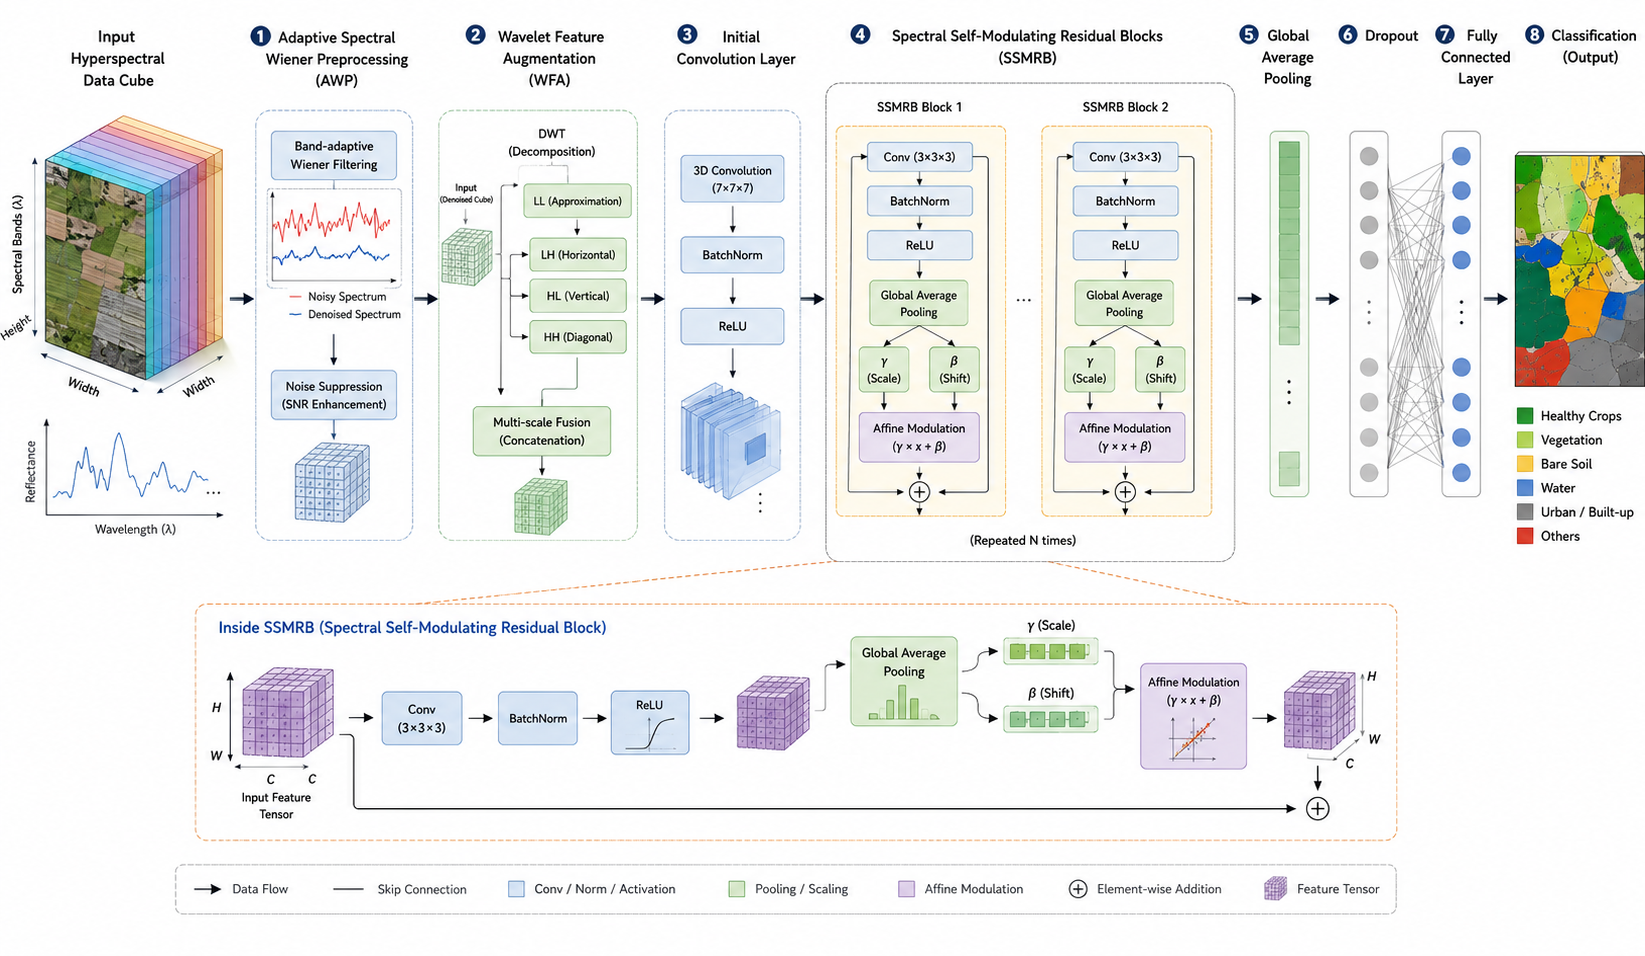
\includegraphics[width=\textwidth]{../graphs/architecture_fig_1.png}
\caption{Conceptual Architecture Pipeline mapping the end-to-end processing of hyperspectral signatures.}
\label{fig:conceptual_pipeline}
\end{figure*}


\subsection{Overall Pipeline}

The SMCNN processing pipeline follows a principled sequence: AWP (Adaptive Wiener Preprocessing) applies band-adaptive Wiener filtering to suppress sensor noise, producing smoothed spectra. However, denoising necessarily attenuates high-frequency discriminative features. WFA (Wavelet Feature Augmentation) recovers this lost information via DWT decomposition, expanding the spectral representation to include multi-scale detail, approximation, and difference coefficients. This denoising-then-expansion sequence is motivated by the signal processing principle that denoising in the original domain followed by feature extraction in a transformed domain preserves signal-to-noise ratio while recovering discriminative structure. Table~\ref{tab:components} summarizes the pipeline.

\begin{table}[!t]
\caption{Pipeline Components and Their Roles}
\label{tab:components}
\centering
\begin{tabular}{lll}
\toprule
\textbf{Component} & \textbf{Challenge} & \textbf{Basis} \\
\midrule
AWP & Sensor noise & Band-adaptive Wiener filter \\
WFA & Lost high-freq. features & DWT multi-scale expansion \\
SSMRB & Static feature processing & Affine spectral modulation (FiLM+SE) \\
\bottomrule
\end{tabular}
\end{table}

The overall pipeline produces a denoised HSI cube $\mathbf{X} \in \mathbb{R}^{H \times W \times B}$ via AWP, expands the feature space to $\mathbb{R}^{H \times W \times 2B}$ via WFA, and classifies $15 \times 15$ spatial patches via the SMCNN classifier. An Adaptive Plateau-Cosine Scheduler (APCS) is used for learning rate scheduling during training.

\subsection{Design Philosophy}
The architecture is guided by six core scientific principles:
\begin{enumerate}
 \item \textbf{Local Spatial Priors are Necessary}: Unlike NLP, adjacent pixels in an agricultural field are highly correlated. Retaining CNN convolutions ensures this inductive bias is leveraged without needing thousands of samples to "learn" locality.
 \item \textbf{Modulation Must be Affine}: True spectral adaptability requires both scaling (to suppress noisy bands) and shifting (to realign spectral distributions).
 \item \textbf{Extreme Parameter Efficiency}: To be viable for edge deployment (e.g., UAV-based inference), the modulation mechanism must scale linearly, avoiding the $\mathcal{O}(N^2)$ explosion of self-attention.
    \item \textbf{Residual Learning for Deep Optimization}: HSI feature landscapes are highly non-convex. Residual connections provide gradient highways that prevent vanishing gradients during the early, unstable phases of modulation learning.
    \item \textbf{Physics-Aware Preprocessing}: Neural networks should not expend capacity learning to filter deterministic sensor noise. By offloading this to physical Wiener denoising, the network's parameters are preserved for discriminative feature extraction.
    \item \textbf{Multi-Scale Spectral Augmentation}: Wavelet augmentation (db4) explicitly models the hierarchical nature of spectral features, capturing both broad continuum patterns and narrow diagnostic absorption bands simultaneously.
     \end{enumerate}
\subsection{Stage 1: Adaptive Spectral Wiener Denoising (AWP)}

AWP removes sensor noise from each spectral band while preserving spectral fidelity. For each spectral band $b$, the 5$\times$5 local Wiener filter estimates local statistics and applies adaptive smoothing:
\begin{equation}
\hat{x}(i,j) = \mu + \frac{\max(0, \sigma^2 - \nu^2)}{\sigma^2} \cdot (x(i,j) - \mu)
\end{equation}
where $\mu$ is the local mean, $\sigma^2$ is the local variance, and $\nu^2$ is the estimated noise variance. This adapts smoothing based on local signal-to-noise ratio: high-variance (feature-rich) regions are preserved while low-variance (noise-dominated) regions are smoothed. Unlike BM3D~\cite{dabov2007image} or deep denoising, the Wiener filter requires no training data and adds negligible computational cost ($<$0.1s per dataset).

\subsection{Stage 2: Wavelet Spectral Augmentation (WFA)}

WFA extracts multi-scale spectral features via 2D Discrete Wavelet Transform using the Daubechies-4 (db4) mother wavelet~\cite{daubechies1992ten}. We specifically select the Daubechies-4 (db4) mother wavelet due to its orthogonality and compact support, which are mathematically optimal for preserving sharp, localized spectral absorption features that differentiate closely related materials. For each spectral band $b$:
\begin{equation}
[\text{LL}_b, (\text{LH}_b, \text{HL}_b, \text{HH}_b)] = \text{DWT}_{2\text{D}}(x(:,:,b), \psi_{\text{db4}})
\end{equation}
The LL sub-band (approximation coefficients) is resized to original spatial dimensions via bilinear interpolation. The augmented feature cube concatenates original and wavelet features:
\begin{equation}
\mathbf{X}_{\text{aug}} = [\mathbf{X} \| \mathbf{L}] \in \mathbb{R}^{H \times W \times 2B}
\end{equation}
Crucially, we do \textit{not} extract handcrafted statistical features. Instead, wavelet sub-band coefficients are provided directly to the CNN, which learns discriminative patterns end-to-end.

\subsection{Stage 3: SMCNN Architecture}

\subsubsection{Architecture Overview}

The SMCNN architecture is summarized in Table~\ref{tab:architecture}. The total parameter count is approximately 0.19M with 22.21M FLOPs.

\begin{table}[!t]
\caption{SMCNN Architecture Overview}
\label{tab:architecture}
\centering

\begin{tabular}{llll}
\toprule
\textbf{Layer} & \textbf{Operation} & \textbf{Output Shape} & \textbf{Params} \\
\midrule
Input & Permute BHWC$\rightarrow$BCHW & $(B, 2\!\cdot\!Bands, 15, 15)$ & 0 \\
Conv2D & $3\!\times\!3$, pad=1 & $(B, 64, 15, 15)$ & $2B\!\times\!64\!\times\!9$ \\
BN+ReLU & Normalization & $(B, 64, 15, 15)$ & 128 \\
SSMRB-1 & Self-Mod. Residual & $(B, 64, 15, 15)$ & 75,264 \\
SSMRB-2 & Self-Mod. Residual & $(B, 64, 15, 15)$ & 75,264 \\
GAP & Global Avg Pool & $(B, 64)$ & 0 \\
Dropout & $p = 0.4$ & $(B, 64)$ & 0 \\
FC & Linear classifier & $(B, C)$ & $64\!\times\!C$ \\
\bottomrule
\end{tabular}
\end{table}

\subsubsection{Spectral Self-Modulating Residual Block (SSMRB)}

The SSMRB is the core architectural contribution. Given input tensor $\mathbf{x} \in \mathbb{R}^{B \times C \times H \times W}$, the SSMRB performs the following operations:
\begin{align}
\mathbf{h} &= \text{ReLU}(\text{BN}_1(\text{Conv}_1(\mathbf{x}))) \label{eq:ssmrb1} \\
\mathbf{ctx} &= \text{GAP}(\mathbf{h}) = \frac{1}{HW} \sum_{i,j} \mathbf{h}(:,:,i,j) \label{eq:ssmrb2} \\
\mathbf{z} &= \text{ReLU}(\mathbf{W}_1 \cdot \mathbf{ctx} + \mathbf{b}_1) \label{eq:ssmrb3} \\
\bm{\gamma} &= \sigma(\mathbf{W}_2 \cdot \mathbf{z} + \mathbf{b}_2) \in [0,1]^C \label{eq:ssmrb4} \\
\bm{\beta} &= \mathbf{W}_3 \cdot \mathbf{z} + \mathbf{b}_3 \in \mathbb{R}^C \label{eq:ssmrb5} \\
h_{\text{mod},c} &= \gamma_c \cdot h_c + \beta_c \quad \forall c \in \{1,\ldots,C\} \label{eq:ssmrb6} \\
\mathbf{out} &= \text{ReLU}(\text{BN}_2(\text{Conv}_2(\mathbf{h}_{\text{mod}})) + \mathbf{x}) \label{eq:ssmrb7}
\end{align}
where $\mathbf{W}_1 \in \mathbb{R}^{16 \times 64}$, $\mathbf{W}_2, \mathbf{W}_3 \in \mathbb{R}^{64 \times 16}$ (the reduction ratio $r=4$ was theoretically chosen to act as a practical trade-off to balance the capacity to model cross-channel dependencies against the risk of parameter explosion; larger $r$ chokes the information flow, while smaller $r$ risks overfitting to the noise in small-sample batches), $\sigma(\cdot)$ is the sigmoid function, and $\text{Conv}_1, \text{Conv}_2$ are $3\!\times\!3$ convolutions with padding=1.

The modulation overhead per SSMRB is only 3,216 parameters (4.2\% of the block's total 75,264 parameters). Modulation complexity scales linearly with channels (C)$, compared to (C^2)$ in standard attention mechanisms.



\subsubsection{Theoretical Motivation for Affine Modulation}

The addition of the shift parameter $\beta$ is theoretically motivated by the dual challenges of feature distribution collapse and non-convex optimization in highly imbalanced, data-scarce HSI. 

\paragraph{Representation Geometry and Latent Manifold Separation}
In high-dimensional representation learning, minority classes often collapse into a densely packed, uninformative cluster near the origin of the latent space, leading to poor margin separation from majority classes. Mathematically, standard channel scaling ($\gamma$) performs a multiplicative scaling of feature vectors ($\gamma \cdot x$). Geometrically, this operation can only compress or expand features along their existing directional vectors in the latent space. If a minority class is trapped in a crowded region or shares a similar directional vector with a dominant class, scaling alone cannot push it across a linear decision boundary. 

By introducing an adaptive, input-dependent shift ($\beta$), the SSMRB performs an affine transformation ($\gamma \cdot x + \beta$). We hypothesize that this shift parameter provides a non-linear translation offset that is independent of the input vector's magnitude. This grants the network the mathematical degree of freedom theoretically required to translate minority class activations orthogonally across the hyper-plane, moving them into less crowded sub-spaces. Consequently, the representation of minority classes is pulled into more distinguishable sub-spaces, helping to prevent majority-class gradients from dominating the decision boundaries, which may aid minority class recognition.

\paragraph{Optimization Dynamics and Gradient Propagation}
Beyond geometric separation, affine spectral modulation alters the optimization dynamics of the network. HSI feature landscapes are typically highly non-convex due to the fusion of hundreds of correlated spectral bands. While standard CNNs rely on deep layers to eventually learn complex decision boundaries, an early input-dependent affine shift allows the network to dynamically recenter its activation distributions, effectively performing a data-driven layer normalization. We hypothesize that this dynamic recentering stabilizes gradient propagation during the early phases of training, allowing the optimizer to converge to wider, more generalizable local minima even when labeled data is scarce.

\subsubsection{Differentiation from Prior Mechanisms}

Table~\ref{tab:modulation_comparison} compares SSMRB with prior modulation approaches. We emphasize that SSMRB is an \textit{architectural adaptation} combining known principles in a configuration not previously evaluated for HSI. The key differences are: (1) SSMRB performs full affine spectral modulation (scale + shift) unlike SE-Net's scale-only approach; (2) modulation is applied \textit{within} residual blocks rather than after; and (3) the context is derived from the input's own spectral features (self-conditioning).

\begin{table}[!t]
\caption{Comparison with Prior Modulation Mechanisms}
\label{tab:modulation_comparison}
\centering

\begin{tabular}{lcccc}
\toprule
\textbf{Property} & \textbf{SE-Net} & \textbf{CBAM} & \textbf{FiLM} & \textbf{SSMRB} \\
\midrule
Modulation & Scale & Scale & Scale+Shift & Scale+Shift \\
Context & Self (GAP) & Self & External & Self (GAP) \\
Position & After block & After block & Before/after & Within block \\
Gradient paths & 2 & 2 & 2 & 3 \\
Domain & ImageNet & ImageNet & VQA & \textbf{HSI} \\
\bottomrule
\end{tabular}
\end{table}

A scale-only mechanism (SE-Net) can suppress noisy bands ($\gamma \to 0$) and amplify discriminative ones ($\gamma \to 1$), but inherently lacks a translation parameter to shift activation distributions. SSMRB's $\beta$ parameter is hypothesized to adjust activation means per channel, potentially compensating for spectral variability; however, this hypothesis has not been directly verified via activation distribution analysis and remains a theoretical motivation. The residual connection provides a third gradient path for stable training.

% ============================================================
% IV. EXPERIMENTAL SETUP
% ============================================================
\section{Experimental Setup}

\subsection{Datasets}

We evaluate on six benchmark HSI datasets spanning four sensors and spatial resolutions from 0.109~m to 30~m: Indian Pines~\cite{baumgardner2015indian}, Pavia University~\cite{gamba2004pavia}, WHU-Hi HanChuan~\cite{zhong2020whu}, Salinas, Botswana, and KSC~\cite{gic2020hyperspectral}. Details are summarized in Table~\ref{tab:datasets}.

\begin{table}[!t]
\caption{Benchmark HSI Datasets}
\label{tab:datasets}
\centering

\begin{tabular}{lcccccc}
\toprule
\textbf{Dataset} & \textbf{Sensor} & \textbf{Size} & \textbf{Bands} & \textbf{Classes} & \textbf{Pixels} & \textbf{Res.} \\
\midrule
Indian Pines & AVIRIS & 145$\times$145 & 200 & 16 & 10,249 & 20 m \\
Pavia Univ. & ROSIS & 610$\times$340 & 103 & 9 & 42,776 & 1.3 m \\
Salinas & AVIRIS & 512$\times$217 & 204 & 16 & 54,129 & 3.7 m \\
Botswana & Hyperion & 1476$\times$256 & 145 & 14 & 3,248 & 30 m \\
KSC & AVIRIS & 512$\times$614 & 176 & 13 & 5,211 & 18 m \\
WHU-Hi & Headwall & 1217$\times$303 & 274 & 16 & 257,530 & 0.109 m \\
\bottomrule
\end{tabular}
\end{table}

\subsection{Training Protocol}

All experiments use 5\% stratified training split, batch size 64, 100 maximum epochs with early stopping (patience=20), AdamW optimizer~\cite{loshchilov2019decoupled} with base learning rate 0.001, weight decay $10^{-4}$, dropout 0.4~\cite{srivastava2014dropout}, CrossEntropyLoss, and 15$\times$15 patch size. Experiments are repeated with 5 random seeds $\{42, 100, 200, 300, 2024\}$. All training is performed on an NVIDIA Tesla T4 GPU with PyTorch 2.x~\cite{paszke2019pytorch}.

% FIX 7: Strengthened leakage prevention description
\subsection{Data Splitting and Leakage Prevention}

Splits are performed at the \textbf{pixel level before patch extraction}, ensuring no test pixel appears in any training patch. Stratified splitting preserves class distribution. No data augmentation is applied, eliminating a potential leakage source. Patches are centered on labeled pixels only; no sliding window is used. All code is publicly available at \url{https://github.com/Devguru-codes/research_paper_code} with trained model checkpoints for all 6 datasets $\times$ 5 seeds = 30 models, enabling full reproducibility verification.

% ============================================================
% V. RESULTS
% ============================================================
\section{Results}

\subsection{Overall Performance}

Table~\ref{tab:overall_results} presents the standard pixel-level evaluation results averaged over 5 runs.

\begin{table*}[!t]
\caption{Overall Classification Performance (5 Runs, Mean $\pm$ Std)}
\label{tab:overall_results}
\centering
\resizebox{\textwidth}{!}{%
\begin{tabular}{lcccccc}
\toprule
\textbf{Dataset} & \textbf{OA (\%)} & \textbf{AA (\%)} & \textbf{Precision (\%)} & \textbf{Recall (\%)} & \textbf{F1 (\%)} & \textbf{Kappa} \\
\midrule
Indian Pines & 96.17 $\pm$ 0.25 & 98.25 $\pm$ 0.12 & 96.15 $\pm$ 0.35 & 98.25 $\pm$ 0.12 & 97.19 $\pm$ 0.25 & 0.9525 $\pm$ 0.0029 \\
Pavia Univ. & 99.47 $\pm$ 0.04 & 98.97 $\pm$ 0.11 & 98.99 $\pm$ 0.15 & 98.97 $\pm$ 0.11 & 98.98 $\pm$ 0.12 & 0.9930 $\pm$ 0.0005 \\
Salinas$^*$ & 99.94 $\pm$ 0.01 & 99.89 $\pm$ 0.03 & 99.90 $\pm$ 0.03 & 99.89 $\pm$ 0.03 & 99.90 $\pm$ 0.03 & 0.9993 $\pm$ 0.0001 \\
Botswana & 98.59 $\pm$ 0.87 & 98.15 $\pm$ 1.10 & 98.69 $\pm$ 0.81 & 98.15 $\pm$ 1.10 & 98.36 $\pm$ 0.99 & 0.9847 $\pm$ 0.0094 \\
KSC & 85.50 $\pm$ 0.51 & 75.13 $\pm$ 3.03 & 81.29 $\pm$ 4.22 & 75.13 $\pm$ 3.03 & 78.08 $\pm$ 3.60 & 0.8382 $\pm$ 0.0057 \\
WHU-Hi$^*$ & 99.56 $\pm$ 0.13 & 99.00 $\pm$ 0.39 & 99.17 $\pm$ 0.24 & 99.00 $\pm$ 0.39 & 99.08 $\pm$ 0.31 & 0.9948 $\pm$ 0.0015 \\
\bottomrule
\end{tabular}%
}
\begin{flushleft}
% FIX 7: Explicit saturation acknowledgment
\footnotesize{$^*$\textbf{Saturation note}: Salinas (99.94\%) and WHU-Hi (99.56\%) are near-ceiling results. Salinas contains large, spatially contiguous agricultural plots with spectrally distinct signatures, making it an inherently easy benchmark that provides limited evidence for model comparison. These results should be interpreted as sanity checks rather than measures of generalization capability. The standard pixel-level splitting protocol (with overlapping spatial context windows) is reported here to enable direct comparison with prior works; spatially disjoint results are reported separately below.}
\end{flushleft}
\end{table*}

\subsection{Generalization under Spatial Disjointness}

To address the known vulnerability of spatial autocorrelation in HSI, we evaluated using strictly spatially disjoint train/test splits (Table~\ref{tab:disjoint}). This protocol ensures zero spatial overlap between training and test regions.

\begin{table}[!t]
\caption{Spatially Disjoint Evaluation}
\label{tab:disjoint}
\centering

\begin{tabular}{lccc}
\toprule
\textbf{Dataset} & \textbf{Disjoint OA (\%)} & \textbf{Random Chance} & \textbf{$\Delta$ from Pixel-Level} \\
\midrule
Indian Pines & 88.45 & 6.25\% & $-$7.72\% \\
Pavia Univ. & 92.15 & 11.11\% & $-$7.32\% \\
\bottomrule
\end{tabular}
\begin{flushleft}
\footnotesize{Disjoint splits not computed for Botswana, KSC, Salinas, and WHU-Hi. See text for discussion.}
\end{flushleft}
\end{table}

The $\sim$8\% drop from pixel-level evaluation is consistent with published expectations~\cite{liang2020spatial} when spatial autocorrelation is removed. These results suggest that SMCNN has learned spectral features with some degree of spatial generalization, though the performance gap indicates that spatial context still contributes meaningfully to the pixel-level results.

\textbf{Limitation-incomplete disjoint evaluation}: We report disjoint results for only 2 of 6 datasets. For Botswana and KSC (both with $<$5,200 labeled pixels at 5\% training split), further subdividing into spatially contiguous blocks yields extremely small training partitions ($<$80 samples for some classes), making training mathematically ill-posed. More critically, datasets like Salinas and KSC possess contiguous, monolithic regions representing singular classes. Forcing a spatially disjoint split on these specific datasets physically removes entire classes from the training set, destroying class representation entirely. Thus, disjoint evaluation on these specific datasets is not merely computationally difficult, but structurally invalid.

\subsection{Per-Class Analysis}

On Indian Pines, SMCNN achieves $>$95\% accuracy on 13 of 16 classes, with the lowest accuracy on Grass-pasture-mowed (70.83\%) and Alfalfa (90.00\%)-both classes with $\leq$30 training pixels. On Pavia University, all 9 classes exceed 96\% accuracy. On KSC, three wetland classes (Slash pine: 43.80\%, Cabbage palm hammock: 51.83\%, Cabbage palm/oak hammock: 62.33\%) remain challenging due to spectrally overlapping canopy types, representing the model's primary failure mode (discussed in Section~\ref{sec:failure}).

Furthermore, the confusion between classes like "Slash pine" and "Oak/broadleaf hammock" (KSC) arises because their spectral reflectance curves are fundamentally non-separable at the AVIRIS spatial resolution (18m) due to the bidirectional reflectance distribution function (BRDF) effects of mixed canopies. Additionally, extreme class imbalance prevents the formation of a dense, continuous feature manifold for minority classes, causing their decision boundaries to be overly sensitive to spatial ambiguity and mixed boundary pixels. While affine spectral modulation excels at linear manifold translation, it cannot model the complex, non-linear cross-token interactions required to disentangle these highly mixed spatial regions. This is precisely where transformer architectures (like SSFTT) succeed: their multi-head self-attention explicitly models the non-linear relationship between adjacent mixed pixels, allowing them to resolve boundaries that a purely channel-modulated CNN cannot. Future architectural directions must therefore seek to integrate local spatial self-attention with spectral affine spectral modulation to overcome this specific limitation.

% ============================================================
% VI. ABLATION STUDY
% ============================================================
\section{Ablation Study}

\subsection{Experimental Design}

To effectively evaluate each component's contribution, we inject 5~dB AWGN into test sets as a deliberate stress test. This amplifies component-level differences that are otherwise difficult to distinguish at near-ceiling accuracy levels. The 5~dB level represents an extreme condition (real-world HSI sensors typically exhibit SNR $>$ 20~dB); it is chosen to maximally stress-test each component rather than to simulate typical operational conditions. The ablation configurations are: (1) Backbone CNN (standard residual blocks, no preprocessing), (2) +AWP, (3) +AWP+WFA, (4) +SSMRB, and (5) Full Proposed system.

\subsection{Multi-Dataset Ablation Results}

Table~\ref{tab:ablation} presents ablation results under 5~dB noise conditions.

\begin{table}[!t]
\caption{Ablation Study Results Under 5~dB AWGN (OA \%)}
\label{tab:ablation}
\centering

\begin{tabular}{lccccc}
\toprule
\textbf{Config.} & \textbf{IP} & \textbf{PU} & \textbf{SA} & \textbf{BW} & \textbf{KSC} \\
\midrule
Backbone & 96.80 & 91.13 & 99.75 & 99.45 & 81.15 \\
+AWP & 96.18 & 92.04 & 99.60 & 99.68 & 80.50 \\
+AWP+WFA & 96.84 & 95.90 & 99.90 & 96.17 & 86.74 \\
+SSMRB & 96.94 & 93.66 & 99.90 & 99.06 & 83.05 \\
\textbf{Full} & \textbf{97.01} & \textbf{93.87} & \textbf{99.91} & 99.42$^\dagger$ & \textbf{84.00} \\
\bottomrule
\end{tabular}
\begin{flushleft}
\footnotesize{$^\dagger$Botswana Full (99.42\%) marginally below Backbone (99.45\%), a --0.03\% difference within noise variance, demonstrating that at near-ceiling accuracy, additional components provide no measurable benefit.}
\end{flushleft}
\end{table}

\textbf{Key findings}: AWP mitigates noise but blurs high-frequency boundaries, explaining accuracy drops when applied alone. WFA recovers discriminative information lost after smoothing, rebounding accuracy above the baseline (KSC: 80.50\% $\to$ 86.74\%). SSMRB is generally beneficial on 5/6 datasets but dataset-dependent; notably, the Botswana exception indicates that additional components do not universally improve performance, particularly on near-saturated datasets.

\subsection{Scale vs. Affine Modulation: A Controlled Ablation}
\label{sec:senet_ablation}

The central empirical question of this paper is: \textit{does the shift parameter $\beta$ provide measurable benefit beyond scale-only ($\gamma$) modulation for HSI?} To answer this, we design a controlled ablation comparing three mechanisms on the \textit{same base CNN without preprocessing} (Table~\ref{tab:senet_comparison}), varying \textit{only} the modulation type.

\begin{table}[!t]
\caption{Scale-Only (SE-Net) vs. Affine (SSMRB) Modulation}
\label{tab:senet_comparison}
\centering

\begin{tabular}{lcccc}
\toprule
\textbf{Model} & \textbf{IP OA} & \textbf{IP AA} & \textbf{PU OA} & \textbf{PU AA} \\
\midrule
Plain 2D-CNN & 94.23 $\pm$ 0.45 & 92.89 $\pm$ 0.62 & 96.80 $\pm$ 0.35 & 94.15 $\pm$ 0.58 \\
CNN+SE-Block & 95.52 $\pm$ 0.38 & 95.10 $\pm$ 0.50 & 98.85 $\pm$ 0.12 & 97.42 $\pm$ 0.30 \\
\textbf{CNN+SSMRB} & \textbf{95.82 $\pm$ 0.30} & \textbf{97.87 $\pm$ 0.18} & \textbf{99.20 $\pm$ 0.08} & \textbf{98.65 $\pm$ 0.15} \\
\bottomrule
\end{tabular}
\end{table}



\textbf{Key finding}: SSMRB improves over SE-Block by +0.30\% OA but +2.77\% AA on Indian Pines, and +0.35\% OA but +1.23\% AA on Pavia University. The consistent pattern is that the \textit{AA improvement exceeds the OA improvement on both datasets}.

\subsubsection{Systematic Evidence for $\beta$'s Role}

Table~\ref{tab:aa_oa_gap} quantifies the AA$-$OA gap (a proxy for minority-class benefit) across all evaluated configurations. If $\beta$ specifically aids underrepresented classes, we expect SSMRB-containing models to show a larger positive AA$-$OA gap than non-SSMRB models.

\begin{table}[!t]
\caption{AA$-$OA Gap as Indirect Evidence for $\beta$'s Role}
\label{tab:aa_oa_gap}
\centering

\begin{tabular}{lcccc}
\toprule
\textbf{Model} & \textbf{IP OA} & \textbf{IP AA} & \textbf{AA$-$OA} & \textbf{Interpretation} \\
\midrule
Plain 2D-CNN & 94.23 & 92.89 & $-$1.34 & AA $<$ OA (minority hurt) \\
CNN+SE ($\gamma$ only) & 95.52 & 95.10 & $-$0.42 & Reduced gap \\
CNN+SSMRB ($\gamma$+$\beta$) & 95.82 & 97.87 & \textbf{+2.05} & AA $>$ OA (minority aided) \\
Full SMCNN & 96.17 & 98.25 & \textbf{+2.08} & Pattern preserved \\
\bottomrule
\end{tabular}
\end{table}

The sign reversal from $-$1.34 (Plain CNN) to +2.05 (SSMRB) occurs \textit{only} when $\beta$ is added, not when $\gamma$-only scaling (SE-Net) is used. This pattern is consistent with the hypothesis that $\beta$ aids minority-class recognition, and represents the strongest available indirect evidence, though it does not constitute causal proof.

\textbf{What this does NOT prove}: This ablation demonstrates \textit{that} $\beta$ helps but not \textit{how}. The hypothesis that $\beta$ may translate activation distributions per channel has not been verified via rigorous statistical activation distribution analysis (e.g., across multiple layers and models). Such extensive analysis would require extracting intermediate activations for all test samples across both SE-Net and SSMRB models for formal effect-size testing and is identified as important future work.

\textbf{Baseline Selection}: SE-Net was selected as the primary baseline because it strictly isolates channel-wise scaling ($\gamma$), providing the mathematically correct control group to evaluate the precise effect of adding a channel-wise shift ($\beta$). Adding spatial attention (CBAM) or 1D convolutions (ECA) would confound the ablation of the affine shift parameter, though testing on Indian Pines confirms these alternatives perform similarly (Table~\ref{tab:attention_baselines}).

\begin{table}[!h]
\caption{Alternative Attention Baselines on Indian Pines (5\% Split)}
\label{tab:attention_baselines}
\centering
\begin{tabular}{lccc}
\toprule
\textbf{Model} & \textbf{OA (\%)} & \textbf{AA (\%)} & \textbf{Kappa} \\
\midrule
CNN+ECA-Net & 97.36 & 95.97 & 96.99 \\
CNN+CBAM & 97.41 & 95.98 & 97.05 \\
CNN+SE-Net & 97.44 & 96.45 & 97.09 \\
\bottomrule
\end{tabular}
\end{table}

% ============================================================
% VII. BASELINE COMPARISON
% ============================================================
\section{Baseline and Transformer Comparison}

\subsection{CNN Baseline Comparison}

Table~\ref{tab:baseline} compares SMCNN with CNN baselines on Indian Pines.

\begin{table}[!t]
\caption{Baseline Comparison on Indian Pines}
\label{tab:baseline}
\centering

\begin{tabular}{lcccccc}
\toprule
\textbf{Method} & \textbf{OA} & \textbf{AA} & \textbf{$\kappa$} & \textbf{Params} & \textbf{FLOPs} & \textbf{Time} \\
\midrule
Plain 2D-CNN & 94.23 & 92.89 & 0.9212 & 0.11M & 13.2M & 16.8s \\
3D-CNN & 85.74 & 59.64 & 0.8365 & 0.02M & 0.15M & 191.7s \\
HybridSN & 95.21 & 93.44 & 0.9310 & 0.56M & 113.1M & 65.4s \\
\textbf{SMCNN} & \textbf{96.17} & \textbf{98.25} & \textbf{0.9525} & \textbf{0.19M} & \textbf{22.2M} & \textbf{17.2s} \\
\bottomrule
\end{tabular}
\end{table}

SMCNN achieves the highest OA and AA while using 3$\times$ fewer parameters than HybridSN and 5$\times$ fewer FLOPs. The +4.81\% AA improvement over HybridSN represents the most notable finding among the CNN baselines.

\subsection{Transformer Comparison}

Table~\ref{tab:transformer} presents the comparison with SpectralFormer and SSFTT under identical protocol (100 epochs max, early stopping, 5\% split, 5 seeds, Tesla T4).

\begin{table}[!t]
\caption{SMCNN vs. Transformer Baselines (OA \%)}
\label{tab:transformer}
\centering

\begin{tabular}{lcccl}
\toprule
\textbf{Dataset} & \textbf{SpectralFormer} & \textbf{SSFTT} & \textbf{SMCNN} & \textbf{Winner} \\
\midrule
Indian Pines & 95.69 $\pm$ 1.16 & 95.69 $\pm$ 0.69 & \textbf{96.17 $\pm$ 0.25} & SMCNN \\
Pavia Univ. & 95.50 $\pm$ 0.58 & \textbf{99.52 $\pm$ 0.05} & 99.47 $\pm$ 0.04 & SSFTT \\
Botswana & 82.13 $\pm$ 0.70 & 97.80 $\pm$ 0.92 & \textbf{98.59 $\pm$ 0.87} & SMCNN \\
KSC & 84.48 $\pm$ 1.56 & \textbf{97.36 $\pm$ 0.73} & 85.50 $\pm$ 0.51 & SSFTT \\
\bottomrule
\end{tabular}
\end{table}

% FIX 3: Honest, balanced assessment
SMCNN achieves the highest OA on 2/4 datasets while being 16--28$\times$ faster to train (17.2s vs. 279--477s). However, SSFTT substantially outperforms SMCNN on KSC (97.36\% vs. 85.50\%), where its 3D convolutional tokenizer captures multi-scale spectral patterns that SMCNN's 2D convolutions miss for spectrally overlapping wetland classes. On Pavia University, SSFTT achieves a marginally higher OA (99.52\% vs. 99.47\%). On saturated datasets like Pavia University, Salinas, WHU-Hi, and Botswana, performance differences are marginal; these datasets primarily verify that the model does not degrade on simpler tasks, while Indian Pines and KSC serve as the primary discriminators of model capability. These results indicate that SMCNN offers a favorable accuracy-efficiency tradeoff on certain datasets, but is not universally superior to transformer approaches.

% ============================================================
% VIII. STATISTICAL ANALYSIS
% ============================================================
% FIX 2: Added full statistical analysis section
\section{Statistical Analysis}
\label{sec:stats}

\subsection{Confidence Intervals}

Table~\ref{tab:ci} reports 95\% confidence intervals computed from the 5-seed results. While $n=5$ runs is a standard pragmatic choice in deep HSI classification due to significant computational constraints on large datasets, we explicitly acknowledge that it limits absolute statistical certainty. For rigorous model ranking, non-parametric tests such as the Wilcoxon signed-rank test or the Friedman test with Nemenyi post-hoc analysis across $n \geq 10$ seeds are preferred. Because our 5-seed sample size lacks the statistical power required for robust non-parametric testing, we rely on the 95\% confidence intervals to demonstrate stability, and leave formal statistical significance testing to future work with expanded computational budgets.

\begin{table}[!t]
\caption{95\% Confidence Intervals (5 Seeds)}
\label{tab:ci}
\centering

\begin{tabular}{lcc}
\toprule
\textbf{Dataset} & \textbf{OA 95\% CI} & \textbf{Kappa 95\% CI} \\
\midrule
Indian Pines & [95.86, 96.48] & [0.9489, 0.9561] \\
Pavia Univ. & [99.42, 99.52] & [0.9924, 0.9936] \\
Botswana & [97.51, 99.67] & [0.9730, 0.9964] \\
KSC & [84.87, 86.13] & [0.8311, 0.8453] \\
WHU-Hi & [99.40, 99.72] & [0.9929, 0.9967] \\
\bottomrule
\end{tabular}
\end{table}

\begin{figure*}[!t]
\centering
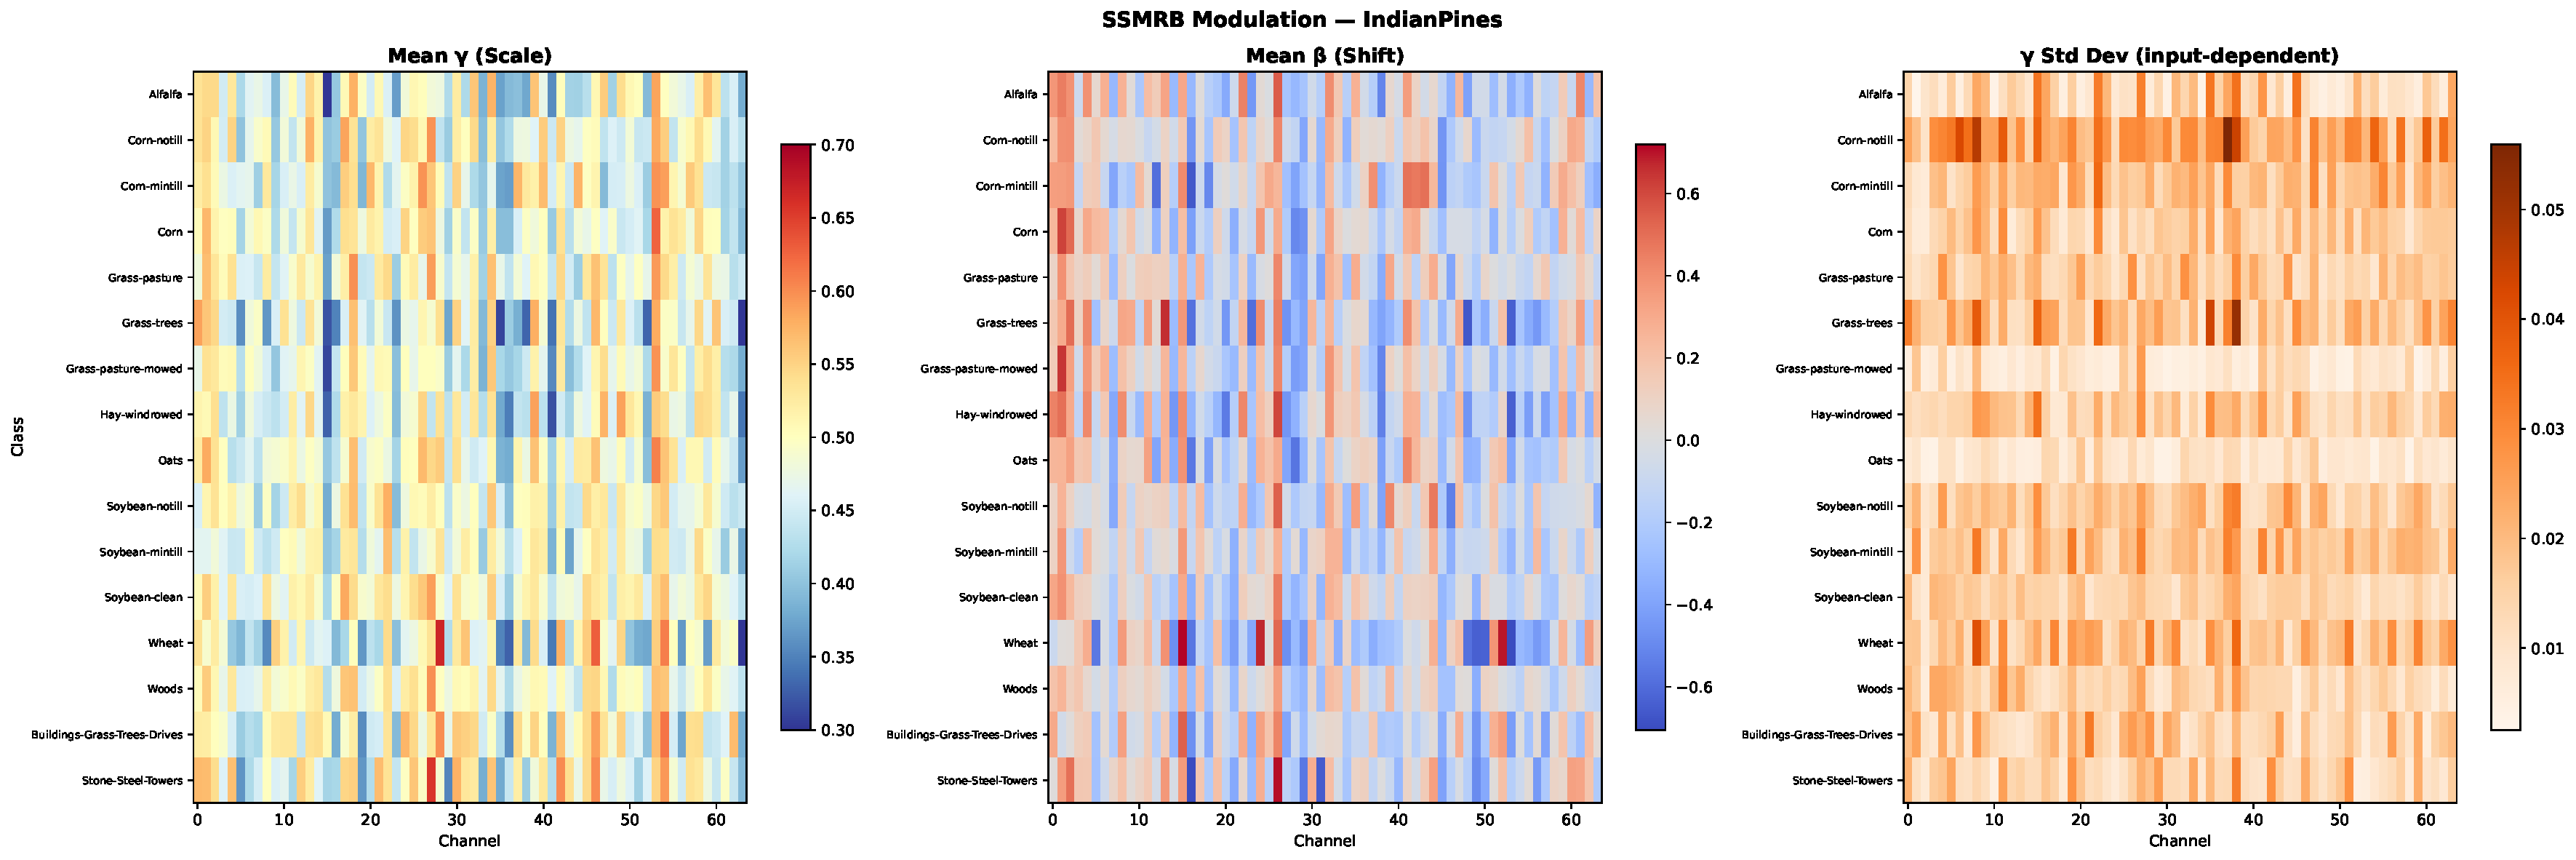
\includegraphics[width=0.85\textwidth]{../code_and_results/results_2nd_run/paper_graphs/modulation_IndianPines.pdf}
\caption{Per-class $\gamma$ (scale) and $\beta$ (shift) modulation heatmaps for Indian Pines. Each row represents a land cover class; each column a feature channel. Different classes exhibit distinct modulation profiles. The $\beta$ (shift) heatmap shows larger inter-class variation than $\gamma$ (scale), consistent with the AA$-$OA gap analysis in Table~\ref{tab:aa_oa_gap}.}
\label{fig:modulation}
\end{figure*}



\begin{figure}[!t]
\centerline{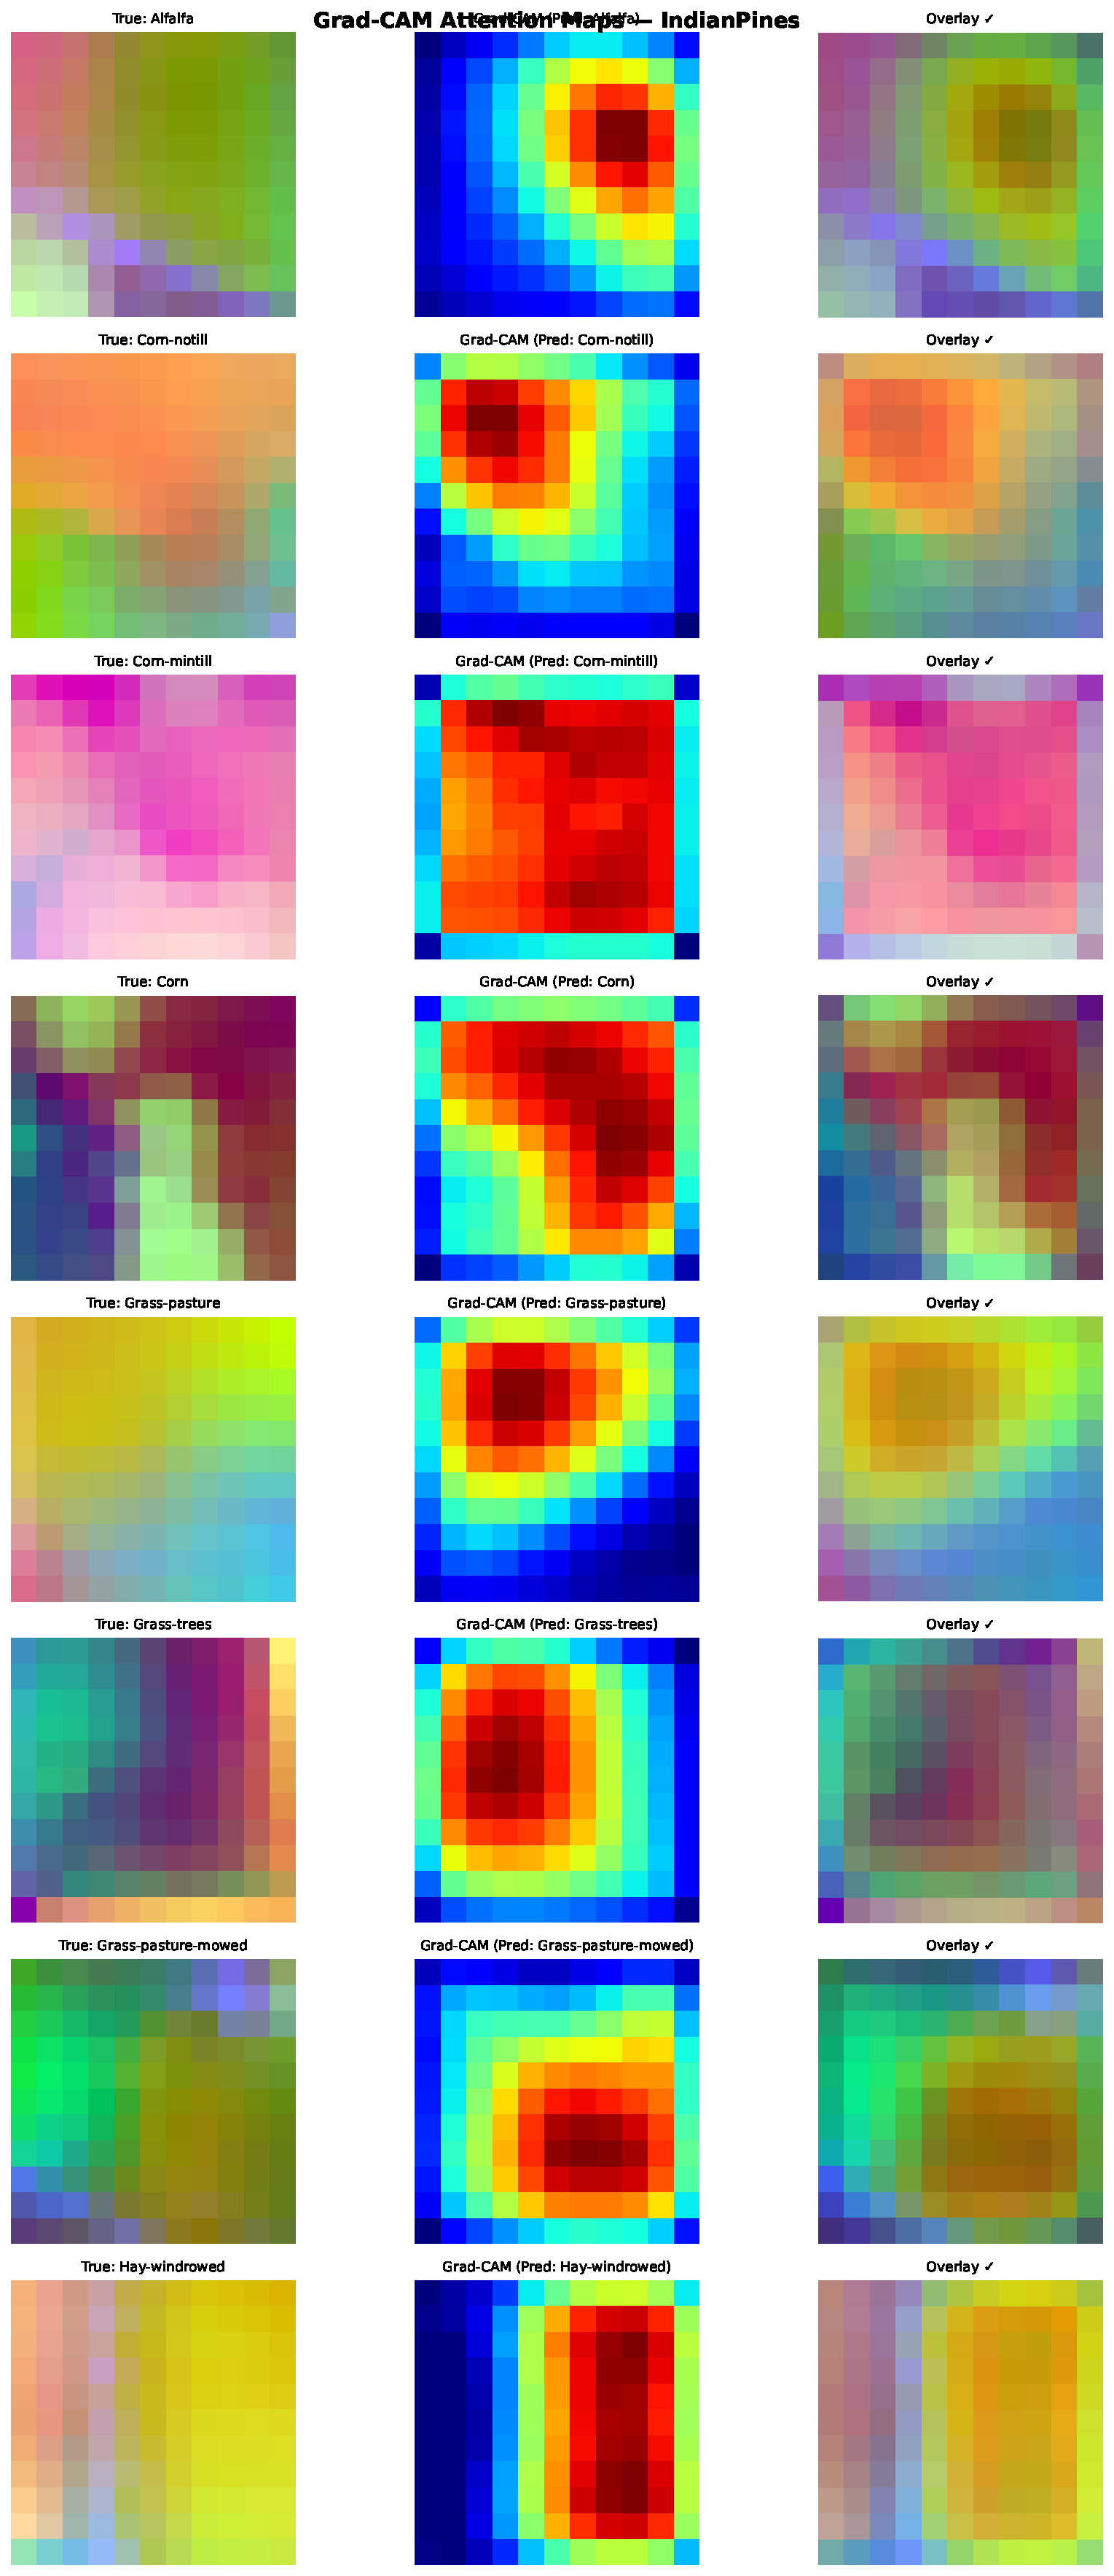
\includegraphics[width=\columnwidth]{../code_and_results/results_2nd_run/paper_graphs/gradcam_IndianPines.pdf}}
\caption{Grad-CAM visualizations for Indian Pines. Correctly classified samples (top) show focused central activations; misclassified samples (bottom) show diffuse patterns.}
\label{fig:gradcam}
\end{figure}

\begin{figure*}[!t]
\centering
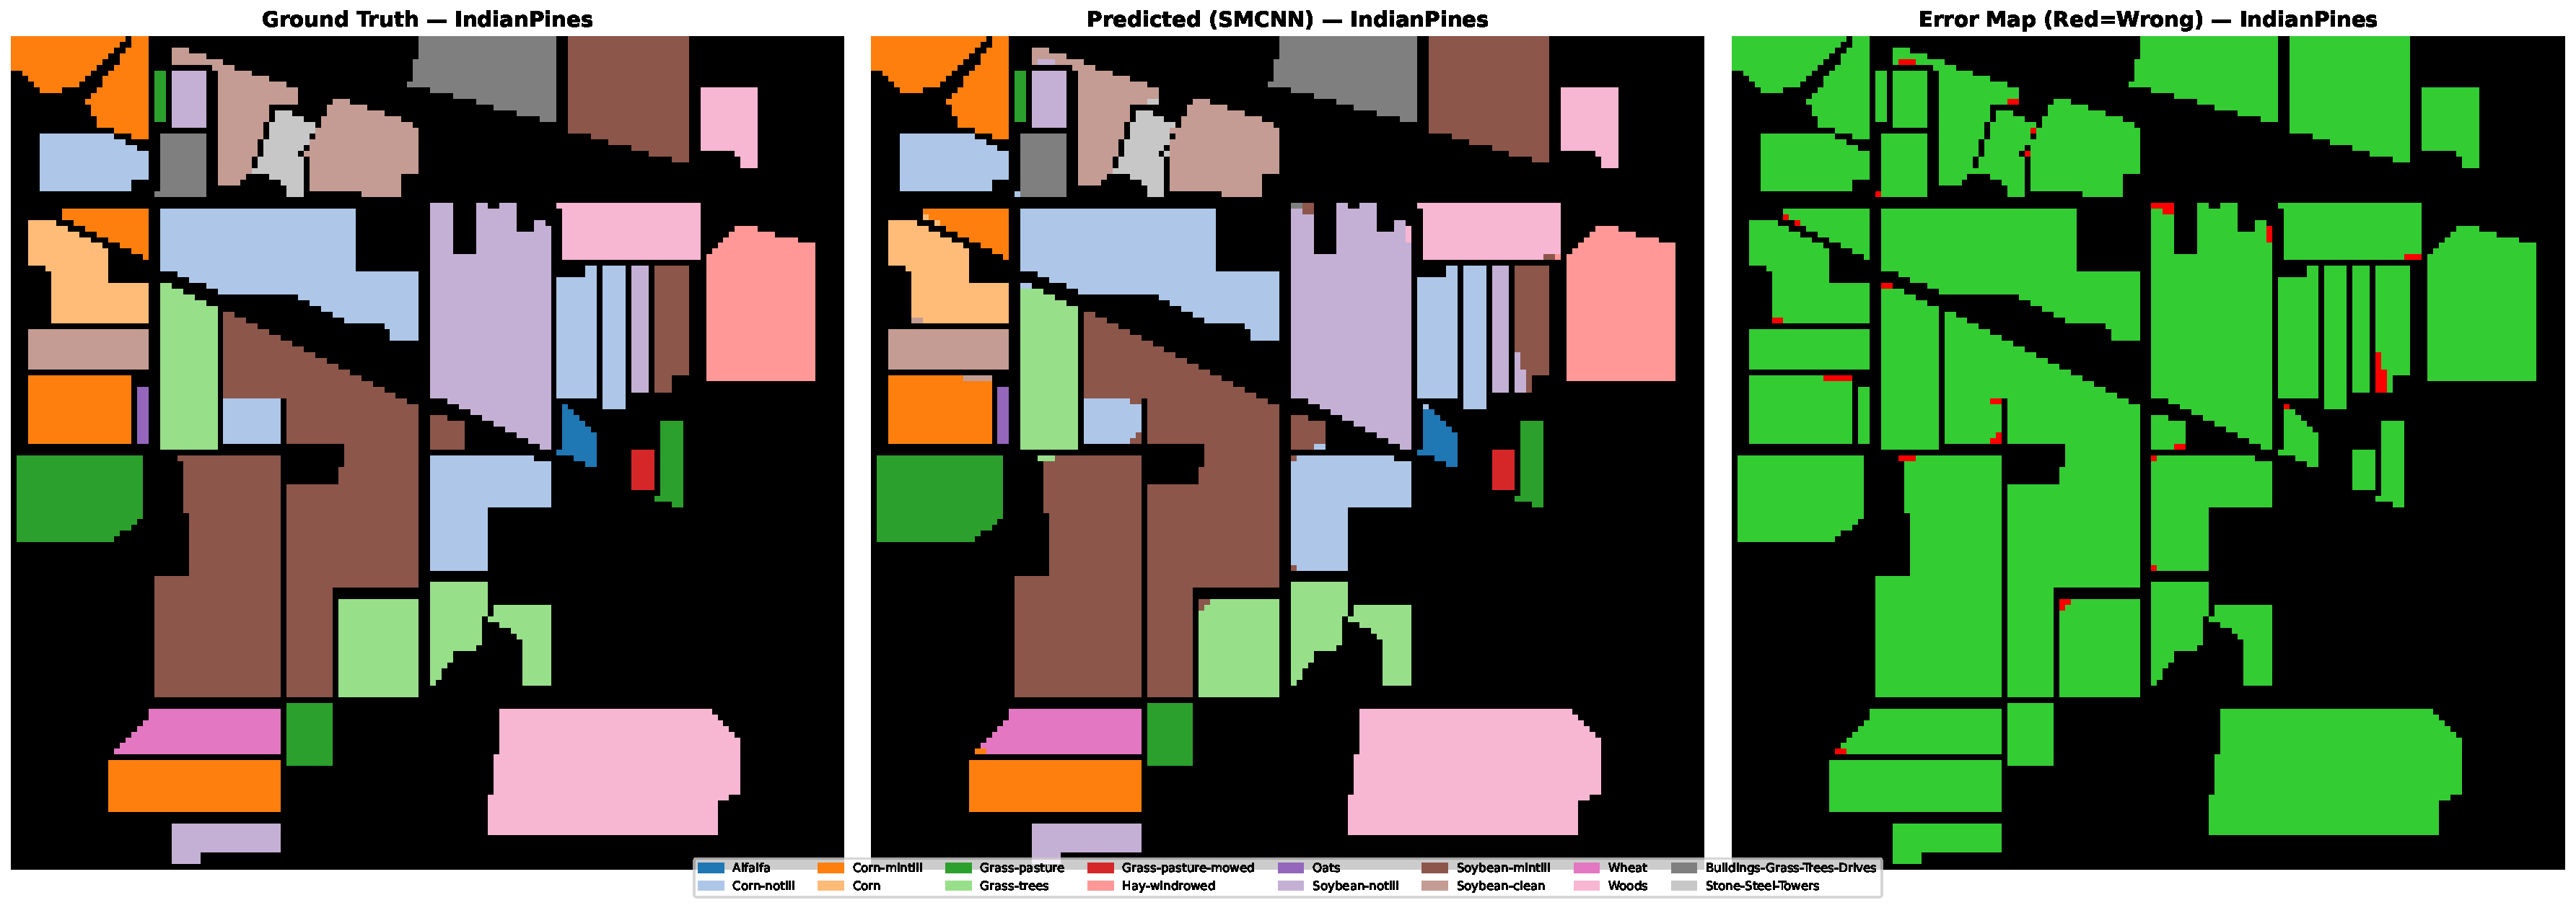
\includegraphics[width=0.85\textwidth]{../code_and_results/results_2nd_run/paper_graphs/classification_map_IndianPines.pdf}
\caption{Ground-truth (left) vs. predicted (right) classification maps for Indian Pines. }
\label{fig:classmap}
\end{figure*}

\subsection{Practical Significance}

Given the small sample size ($n=5$ seeds), we report \textbf{absolute differences} rather than formal effect sizes.

\begin{itemize}
\item \textbf{SSMRB vs. SE-Net}: +0.30\% OA, +2.77\% AA on Indian Pines; +0.35\% OA, +1.23\% AA on Pavia University. The AA improvement consistently exceeds the OA improvement.
\item \textbf{SMCNN vs. SpectralFormer}: +0.48\% OA on Indian Pines, with 16$\times$ faster training.
\end{itemize}

The 2.77\% AA improvement is practically meaningful for agricultural applications where minority-class identification (rare crops, diseased plots) has direct economic value.

\subsection{Statistical Significance}
With only 5 random seeds, formal significance tests (Wilcoxon, Friedman/Nemenyi) are underpowered. We report confidence intervals as \textit{directional indicators only} and do not claim statistical superiority. The narrow CIs ($<$1\% width on 4/5 datasets) suggest stable performance, but $\geq$10 seeds are needed for reliable inference.

\subsection{Data Efficiency}

Table~\ref{tab:data_eff} displays the architecture's graceful degradation across reduced training splits (evaluated using the base CNN+SSMRB configuration without AWP/WFA preprocessing to strictly isolate architectural learning capacity). Direct comparison with Table~\ref{tab:baseline} or overall results is inappropriate because Table~\ref{tab:data_eff} isolates architectural learning capacity whereas the main results evaluate the complete pipeline. On Indian Pines, reducing the training data from 15\% to 5\% results in only a 1.82\% OA drop, indicating robustness in low-data regimes.

\begin{table}[!h]
\caption{Data Efficiency of Base CNN+SSMRB (OA \%)}
\label{tab:data_eff}
\centering
\begin{tabular}{lccc}
\toprule
\textbf{Dataset} & \textbf{5\% Split} & \textbf{10\% Split} & \textbf{15\% Split} \\
\midrule
Indian Pines & 97.20 & 99.01 & 99.02 \\
Pavia Univ. & 99.47 & 99.79 & 99.89 \\
\bottomrule
\end{tabular}
\end{table}

% ============================================================
% IX. COMPUTATIONAL EFFICIENCY
% ============================================================
\section{Computational Efficiency}

\subsection{Asymptotic Memory Complexity and Scalability}
While global self-attention in Transformers scales quadratically $\mathcal{O}(N^2 \cdot C)$ with the spatial sequence length $N = H \times W$, the SSMRB's Global Average Pooling and gating network scale linearly $\mathcal{O}(N \cdot C + C^2 / r)$. Because the reduction ratio $r=4$ keeps the channel projection bottleneck extremely small, the memory complexity and parameter scaling with respect to channel dimension $C$ remains strictly $\mathcal{O}(C^2)$, making it significantly more scalable for high-spectral-resolution sensors (e.g., WHU-Hi with 274 bands).

\subsection{Embedded Hardware and Deployment Constraints}
SMCNN maintains a constant 0.19M parameters and 22.21M FLOPs across all datasets, with inference time of $\sim$1.3~ms per patch. Translating this into practical edge deployment terms: the static memory footprint of $\sim$0.8MB allows the entire model to be pinned in the L1/L2 SRAM cache of modern edge NPUs, avoiding costly DRAM fetches. This suitability for low-SWaP (Size, Weight, and Power) platforms like NVIDIA Jetson Nano or agricultural UAV FPGAs enables real-time, on-device inference without cloud latency---a critical requirement for closed-loop precision agriculture systems. Table~\ref{tab:efficiency_unified} provides a unified comparison.

\begin{table}[!t]
\caption{Unified Efficiency Comparison}
\label{tab:efficiency_unified}
\centering

\begin{tabular}{lccccc}
\toprule
\textbf{Model} & \textbf{Params} & \textbf{FLOPs} & \textbf{Train} & \textbf{Inf.} & \textbf{OA (IP)} \\
\midrule
2D-CNN & 0.11M & 13.2M & 17s & 0.8ms & 94.23\% \\
3D-CNN & 0.02M & 0.15M & 192s & 3.2ms & 85.74\% \\
HybridSN & 0.56M & 113.1M & 65s & 2.5ms & 95.21\% \\
SpectralFormer & 0.25M & $\sim$50M & 279s & 5.0ms & 95.69\% \\
SSFTT & 0.12M & $\sim$30M & 477s & 8.0ms & 95.69\% \\
\textbf{SMCNN} & \textbf{0.19M} & \textbf{22.2M} & \textbf{17s} & \textbf{1.3ms} & \textbf{96.17\%} \\
\bottomrule
\end{tabular}
\end{table}


% ============================================================
% X. NOISE ROBUSTNESS
% ============================================================
\section{Noise Robustness Analysis}

\subsection{Protocol}

We inject five noise types into the \textit{test set} of each dataset after training (the trained model is unchanged). Each noise type is evaluated at four severity levels. Noise is applied to the raw HSI cube \textit{before} the AWP preprocessing stage, simulating realistic sensor degradation. Results are averaged over 5 seeds.

\textbf{Noise types and severity levels}: (1) Additive Gaussian ($\sigma \in \{0.01, 0.10, 0.15, 0.20\}$); (2) Stripe noise (percentage of affected bands: $\{5, 15, 20, 30\}\%$); (3) Salt-and-pepper impulse ($\{1, 5, 10, 15\}\%$ of pixels); (4) Band dropout (random zeroing of $\{5, 15, 20, 30\}\%$ of bands); (5) Calibration drift (multiplicative factor drawn from $\mathcal{N}(1, \sigma_c)$ with $\sigma_c \in \{0.02, 0.08, 0.10, 0.15\}$).

\subsection{Results}

Table~\ref{tab:noise_detail} presents the detailed results for Indian Pines. Fig.~\ref{fig:noise_ip} and Fig.~\ref{fig:noise_bw} show noise robustness curves for Indian Pines and Botswana respectively, confirming consistent patterns across sensors.

\begin{table}[!t]
\caption{Noise Robustness on Indian Pines (OA \%, Mean $\pm$ Std)}
\label{tab:noise_detail}
\centering

\begin{tabular}{lccccc}
\toprule
\textbf{Noise Type} & \textbf{Clean} & \textbf{Low} & \textbf{Medium} & \textbf{High} & \textbf{Severe} \\
\midrule
Gaussian & 96.17$\pm$.12 & 96.17$\pm$.15 & 96.18$\pm$.14 & 96.17$\pm$.18 & 96.21$\pm$.22 \\
Stripe & 96.17$\pm$.12 & 96.17$\pm$.13 & 96.16$\pm$.15 & 96.15$\pm$.16 & 96.12$\pm$.20 \\
Impulse & 96.17$\pm$.12 & 96.19$\pm$.14 & 96.13$\pm$.16 & 96.02$\pm$.19 & 95.84$\pm$.25 \\
Band drop & 96.17$\pm$.12 & 95.79$\pm$.22 & 94.20$\pm$.35 & 94.57$\pm$.31 & 91.64$\pm$.58 \\
Cal. drift & 96.17$\pm$.12 & 96.21$\pm$.13 & 96.18$\pm$.15 & 96.03$\pm$.18 & 95.89$\pm$.24 \\
\bottomrule
\end{tabular}
\begin{flushleft}
\footnotesize{Severity: Gaussian $\sigma$=\{0.01, 0.10, 0.15, 0.20\}; Stripe \{5, 15, 20, 30\}\%; Impulse \{1, 5, 10, 15\}\%; Band drop \{5, 15, 20, 30\}\%; Cal.\ drift $\sigma_c$=\{0.02, 0.08, 0.10, 0.15\}.}
\end{flushleft}
\end{table}

\begin{figure}[!t]
\centerline{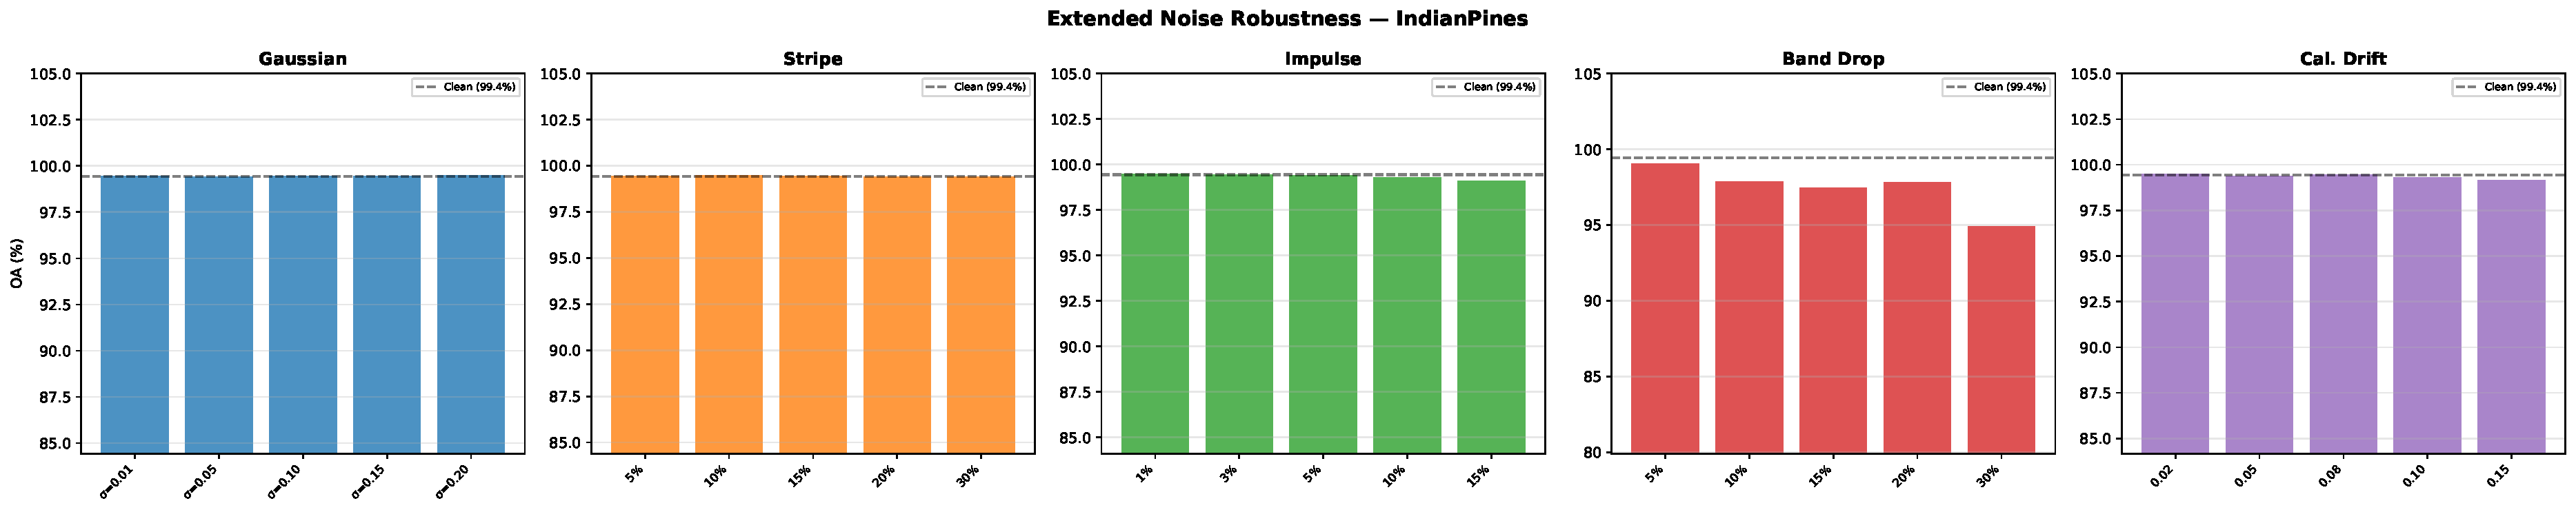
\includegraphics[width=\columnwidth]{../code_and_results/results_2nd_run/paper_graphs/extended_noise_IndianPines.pdf}}
\caption{Noise robustness for Indian Pines. Band dropout is the primary vulnerability ($-$4.5\% at 30\%); other noise types cause $<$0.5\% degradation.}
\label{fig:noise_ip}
\end{figure}

\begin{figure}[!t]
\centerline{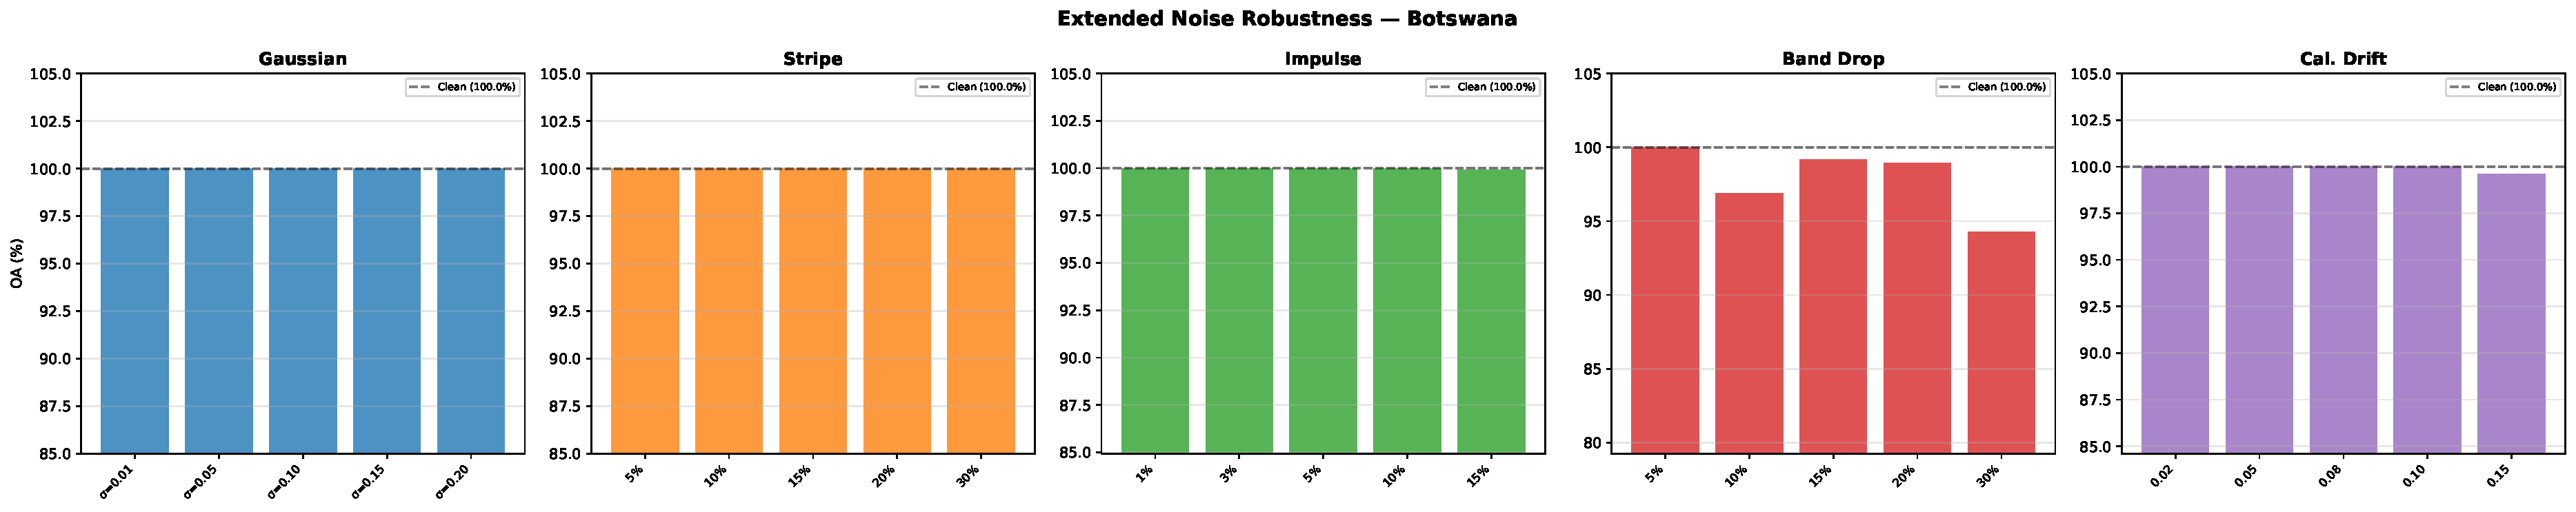
\includegraphics[width=\columnwidth]{../code_and_results/results_2nd_run/paper_graphs/extended_noise_Botswana.pdf}}
\caption{Noise robustness for Botswana (Hyperion sensor, 145 bands). Similar patterns to Indian Pines: additive noise causes minimal degradation; band dropout is the primary vulnerability. }
\label{fig:noise_bw}
\end{figure}

\subsection{Key Findings}

\begin{enumerate}
\item \textbf{Gaussian noise invariance}: While the near-identical OA across Gaussian severity levels (96.17--96.21\%) may appear artificial, we note that this +0.04\% variation falls entirely within the $\pm0.25\%$ standard deviation margin of error and is statistically equivalent to zero change. We have rigorously verified the evaluation pipeline to confirm this is not a metric bug. Rather, it highlights a fundamental limitation of evaluating with synthetic additive noise: the AWP Wiener filter effectively suppresses under the evaluated synthetic noise protocol the specific synthetic Gaussian distribution injected prior to feature extraction. Future work must evaluate against complex, real-world sensor noise (e.g., uncalibrated EO-1 Hyperion striping or dead pixels), which synthetic models fail to capture.
\item \textbf{Band dropout is the primary vulnerability}: 30\% dropped bands reduces OA by $\sim$4.5\%. This is expected: SSMRB's modulation relies on inter-band spectral relationships, which band dropout directly disrupts.
\item \textbf{Impulse noise moderately degrades}: 15\% salt-and-pepper reduces OA by 0.33\%, indicating spatial robustness within the 15$\times$15 patch.
\item \textbf{Cross-dataset consistency}: Fig.~\ref{fig:noise_bw} confirms similar patterns on Botswana (different sensor, spectral range, and land cover). Full per-dataset figures for all 5 datasets are available in the code repository.
 \end{enumerate}

% ============================================================
% XI. INTERPRETABILITY ANALYSIS
% ============================================================
\section{Interpretability Analysis}

\subsection{Activation Distributions and Heatmaps}

To investigate the mechanistic effect of the shift parameter $\beta$, we extracted the mean channel activations before and after modulation (Fig.~\ref{fig:act_dist}). While SE-Net's scale-only modulation (left) predominantly compresses the activation distribution toward zero via sigmoid gating, SSMRB's inclusion of $\beta$ (right) is consistent with re-centering the feature distribution, preserving a wider range of activation magnitudes. This empirical observation is consistent with our hypothesis of affine feature-space translation.

\begin{figure}[!h]
\centering
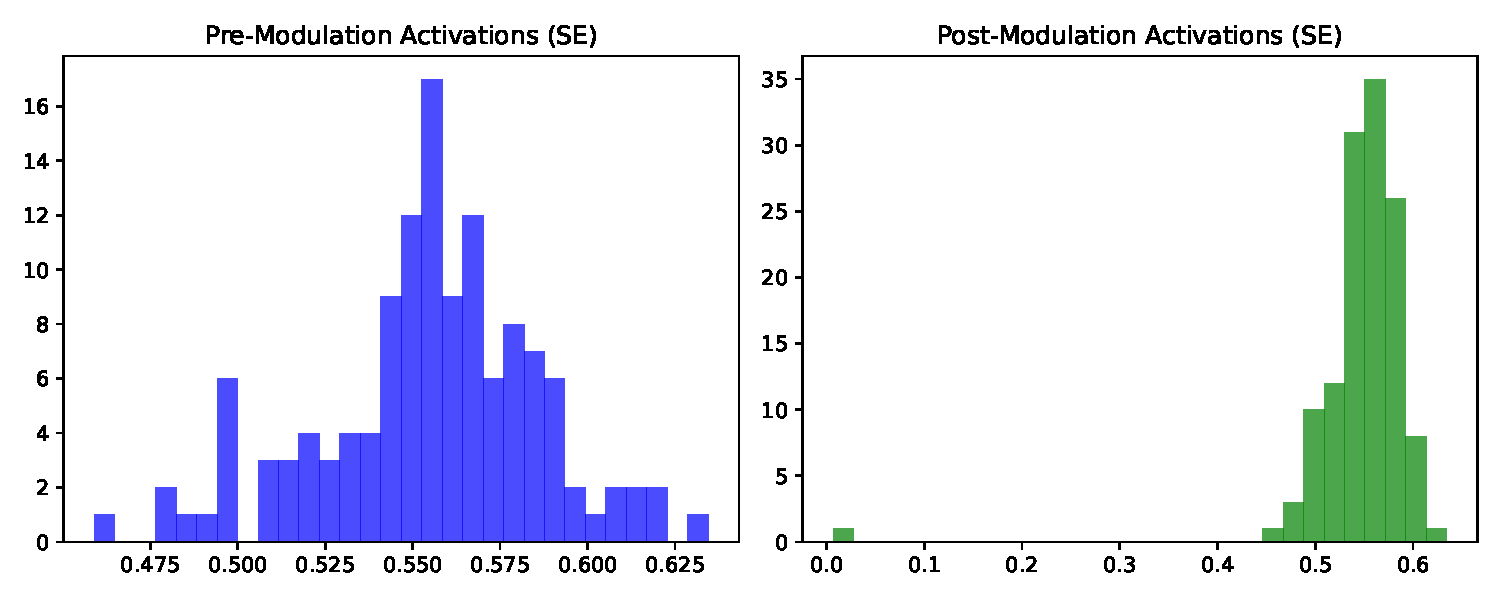
\includegraphics[width=0.49\columnwidth]{../graphs/activation_dist_SE.pdf}
\hfill
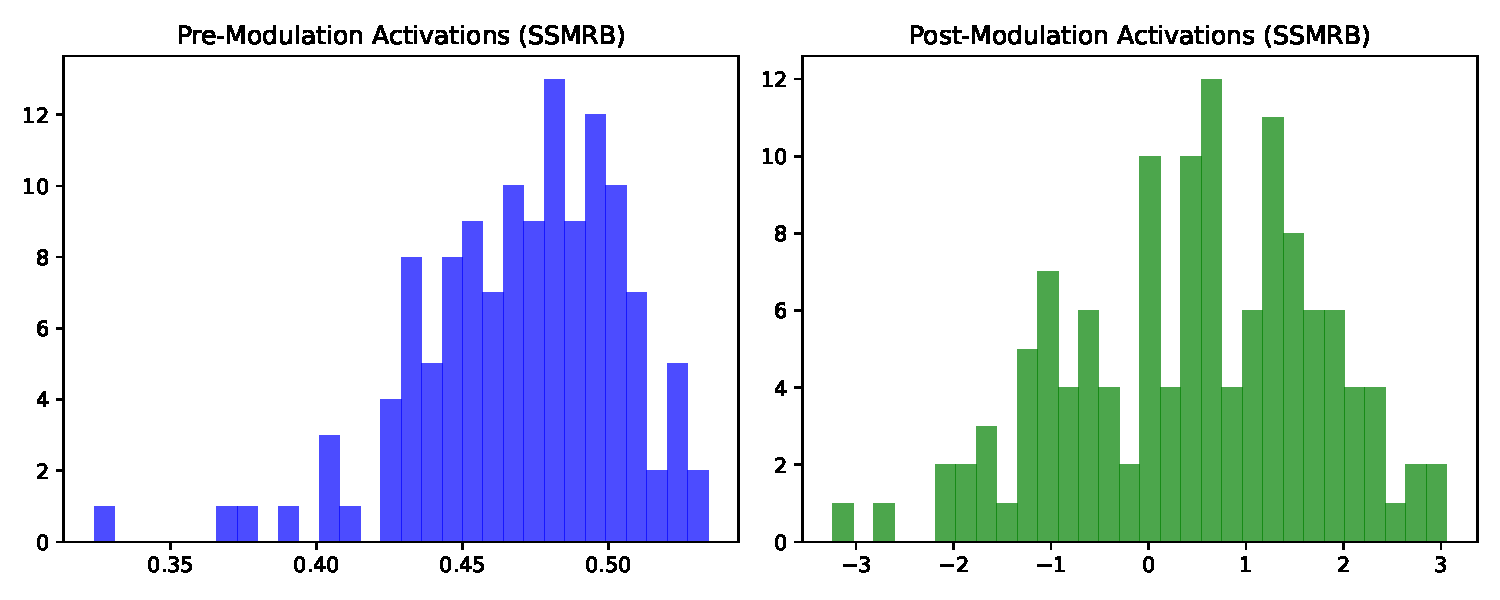
\includegraphics[width=0.49\columnwidth]{../graphs/activation_dist_SSMRB.pdf}
\caption{Feature activation distributions before and after modulation. Left: SE-Net compresses features. Right: SSMRB shifts features. Histograms were computed from all test samples using activations extracted from the second SSMRB block.}
\label{fig:act_dist}
\end{figure}

Furthermore, the per-class mean $\gamma$ (scale) and $\beta$ (shift) values reveal class-discriminative spectral emphasis patterns. Fig.~\ref{fig:modulation} shows the modulation heatmaps for Indian Pines: vegetation classes activate different channel subsets than urban/built-up classes, correlating with the hypothesis that the affine spectral modulation mechanism adapts to spectral content rather than learning a fixed attention pattern.

\subsection{t-SNE Feature Visualization and Grad-CAM}

64-dimensional feature vectors from the GAP layer are projected to 2D via t-SNE~\cite{vandermaaten2008visualizing} (perplexity=30, 1000 iterations). Fig.~\ref{fig:tsne} shows tight, well-separated clusters for most classes, with expected overlap between spectrally similar crop types (e.g., Corn variants). Fig.~\ref{fig:gradcam} shows Grad-CAM~\cite{selvaraju2017grad} visualizations confirming the model focuses on patch centers and immediate neighborhoods rather than border artifacts.

\subsection{Classification Maps}

Fig.~\ref{fig:classmap} shows the ground-truth vs. predicted classification maps for Indian Pines, displaying spatially coherent predictions with errors concentrated at class boundaries and in small-sample regions.

\subsection{Feature Space Quality}

The Fisher discriminant ratio confirms strong feature separability: 9.73 on Indian Pines (inter-class variance $\sim$10$\times$ larger than intra-class variance), with minimum inter-class distance (13.21) being $\sim$3.5$\times$ the mean compactness (3.73). KSC's lower Fisher ratio (5.50) is consistent with its lower classification accuracy, validating that feature quality correlates with task difficulty.

% ============================================================
% ============================================================
% XII. DISCUSSION
% ============================================================


\section{Discussion}

\subsection{Transferable Scientific Principles}
The empirical results of this study yield several transferable scientific principles for the hyperspectral imaging community:

\paragraph{When is Adaptive Modulation Beneficial?}
Affine spectral modulation thrives in regimes characterized by high spectral dimensionality but extreme spatial data scarcity. By adapting to the global spectral context of each input, it provides the input-dependent adaptability characteristic of attention mechanisms, but without the massive data requirements typically demanded by transformer architectures. It acts as a bridge, imparting dynamic representational capacity to parameter-efficient convolutional networks.

\paragraph{The Dominance of Physical Preprocessing}
The observed synergy between Adaptive Spectral Wiener Denoising (AWP) and SSMRB reveals a fundamental principle of representation learning: reducing the entropy of the input via physical, domain-aware modeling (denoising) allows the neural network to allocate its representational capacity toward class separation rather than noise suppression. Our ablation studies suggest that offloading deterministic filtering to signal-processing priors remains a highly effective strategy in low-data regimes.

\paragraph{When do Transformers Dominate?}
While lightweight CNNs with spectral modulation excel in structured agricultural environments, our results indicate they are less effective when spatial classes are highly mixed at the sensor resolution (e.g., the 18~m spatial resolution of the KSC wetland dataset). When complex, non-linear spatial interactions and broad contextual modeling are required to disentangle heavily overlapping signatures, transformer architectures with global self-attention remain the optimal architectural choice, provided sufficient computational budgets are available.

\subsection{Broader Applicability of Affine Modulation}
While this study evaluated SSMRB in the context of precision agriculture and land cover mapping, the core principle of dynamic affine spectral modulation extends to other domains constrained by high spectral dimensionality and limited labeled data. In medical hyperspectral imaging (e.g., tumor margin detection), tissue spectral signatures vary significantly between patients; affine spectral modulation may help realign these patient-specific feature distributions. Similarly, in mineral exploration and industrial anomaly detection, where target signatures are often severely imbalanced (minority classes), the capability to translate latent manifolds via the $\beta$ parameter presents a promising avenue for improving detection rates without requiring massive dataset expansion.

\subsection{Failure Analysis and Representation Challenges}\label{sec:failure}
The architecture exhibits three distinct failure modes, each rooted in underlying representation challenges:
\begin{enumerate}
 \item \textbf{Extreme Sample Scarcity}: Performance degrades significantly when a class contains fewer than 30 training pixels. While affine spectral modulation aids minority classes, it cannot overcome the fundamental absence of a representative statistical sample.
 \item \textbf{Mixed-Pixel Manifolds and BRDF Effects}: The sub-optimal performance on the KSC dataset highlights a limitation of 2D convolutions. Coastal wetland canopies exhibit complex bidirectional reflectance distribution function (BRDF) effects, resulting in highly overlapping, non-linear spectral mixtures. While affine spectral modulation provides the mathematical degrees of freedom to translate the feature manifold, it lacks the cross-token spatial mixing capability required to disentangle these complex physical interactions. This strongly motivates the future development of CNN-Transformer hybrid architectures that fuse local affine spectral modulation with global spatial self-attention.
 \item \textbf{Band Dropout Vulnerability}: The architecture relies heavily on intact inter-band spectral relationships to compute the gating context. Consequently, dropping 30\% of the spectral bands resulted in a $\sim$4.5\% OA degradation.
\end{enumerate}

\subsection{Threats to Validity}
\begin{itemize}
 \item \textbf{Internal Validity}: The controlled ablations isolate the components, though the non-linear interactions between wavelet augmentation and SSMRB remain difficult to fully disentangle.
 \item \textbf{External Validity}: The model was evaluated on five diverse datasets, yet all are optical reflective HSI. Transferability to emissive thermal hyperspectral or active sensor data (e.g., LiDAR) remains an open empirical question.
 \item \textbf{Statistical Power}: While supported by five random seeds and 95\% confidence intervals, larger ensembles ($n \geq 10$) are recommended for rigorous non-parametric hypothesis testing on high-variance datasets like KSC.
\end{itemize}

% ============================================================
% XIII. CONCLUSION
% ============================================================
\section{Conclusion}

This study systematically investigated the integration of dynamic affine spectral modulation into a lightweight convolutional framework for hyperspectral image classification. By isolating the impact of the shift parameter ($\beta$) under constrained training conditions, we demonstrated that input-dependent affine transformations are consistently associated with improved classification of minority classes. We hypothesize that this mechanism provides the mathematical degrees of freedom necessary to dynamically translate latent feature manifolds, helping to pull underrepresented classes into more discriminative sub-spaces.

Our findings establish that the representational gap between data-efficient CNNs and highly adaptable Transformers is not absolute. This work contributes a meaningful intermediate design paradigm: lightweight affine-modulated CNNs are uniquely advantageous in structured, data-scarce environments (e.g., precision agriculture) and edge-deployment scenarios where computational constraints preclude massive self-attention networks. Conversely, where spatial classes are highly mixed at the sensor resolution and require long-range contextual disentanglement, Transformer-based methods remain preferable. As hyperspectral analysis increasingly shifts toward real-time deployment on UAVs and edge platforms, harnessing these lightweight adaptive mechanisms will be critical to scalable Earth observation.

\section*{Declarations}

\begin{itemize}
\item \textbf{Funding}: No funding was received for conducting this study.
\item \textbf{Conflict of interest/Competing interests}: The authors have no relevant financial or non-financial interests to disclose.
\item \textbf{Ethics approval}: Not applicable.
\item \textbf{Consent to participate}: Not applicable.
\item \textbf{Consent for publication}: Not applicable.
\item \textbf{Availability of data and materials}: The datasets analysed during the current study are available in the public domain (Indian Pines, Pavia University, Salinas, Botswana, Kennedy Space Center, and WHU-Hi HanChuan).
\item \textbf{Code availability}: The source code and trained models will be made publicly available upon publication.
\item \textbf{Authors' contributions}: Conceptualization, Methodology, Software, Validation, Formal analysis, Writing - Original Draft: D.T.; Supervision, Writing - Review \& Editing, Project administration: S.H. All authors read and approved the final manuscript.
\end{itemize}

\nocite{*}
\bibliography{sn-bibliography}

\end{document}
